\documentclass{article}
\usepackage[utf8]{inputenc}
\usepackage[spanish]{babel}

% Necesario para usar fuentes del sistema
% \usepackage{fontspec} 
% \setmainfont{Arial} 

\usepackage{graphicx} % Required for inserting images
\usepackage{imakeidx}
\usepackage{amssymb, amsmath}
\usepackage{listings}
\usepackage{float} % Para poner las imagenes justo donde queramos

\usepackage{xcolor} % Para definir colores personalizados
\usepackage{hyperref}
\usepackage{braket}

% \setlength{\parindent}{0pt} % Elimina la sangría en todo el documento

\numberwithin{equation}{section} % Para las ecuaciones

% Definir un azul más oscuro
\definecolor{darkblue}{rgb}{0.0, 0.0, 1} % Azul oscuro

% Configuración personalizada para hyperref
\hypersetup{
    colorlinks=true,     % Colorear los enlaces en lugar de ponerles un recuadro
    linkcolor=blue,      % Color de los enlaces internos (por ejemplo, índice)
    citecolor=blue,      % Color de los enlaces de citas
    filecolor=magenta,   % Color de los enlaces a archivos
    urlcolor=darkblue        % Color de los enlaces a URLs
}

\makeindex
\setlength{\parindent}{12pt}


% Márgenes de página
\usepackage[left=2.5cm, right=2.5cm, top=3cm, bottom=3cm]{geometry}

% Fuente y formato
\usepackage[T1]{fontenc} % Para las ñ y letras con tilde
\usepackage{times}
\usepackage{microtype} % Mejora el espaciado de las palabras

% Encabezado y pie de página guapo
\usepackage{fancyhdr}
\setlength{\headheight}{12.5pt}
\pagestyle{fancy} 
\fancyhf{} % Limpia los valores predeterminados     
\fancyhead[R]{\textit{\rightmark}} % Sección o subsección actual en la parte superior derecha
\fancyfoot[C]{\thepage} % Número de página centrado en el pie de página

\usepackage{titlesec}  % Paquete para personalizar secciones
\usepackage{tikz}      % Paquete para gráficos y formato personalizado
% Modificar el formato de las secciones
\titleformat{\section}[block]
  {\normalfont\Huge\bfseries\raggedleft}    % Título más grande, en negrita y alineado a la derecha
  {\color{gray}\large CAPÍTULO\\}  % "Capítulo" en gris y pequeño, seguido por el número de la sección
  {\tikz[baseline]{\node[anchor=base, scale=3, text=gray, inner sep=0pt] {\thesection};} \\[1em]}  
  {\normalfont\bfseries\raggedleft}         % Título de la sección en negro, alineado a la derecha
  [\vspace{1em}]                  % Espacio después del título



\begin{document}
    \parindent=0pt

    \begin{titlepage}
        \centering
        {\fontsize{18pt}{22pt}\selectfont \textbf{UNIVERSIDAD ALFONSO X EL SABIO}\par}
        \vspace{1cm}
        {\fontsize{16pt}{22pt}\selectfont \textbf{ESCUELA POLITÉCNICA SUPERIOR}\par}
        \vspace{1cm}
        {\fontsize{14pt}{22pt}\selectfont \textbf{GRADO EN INGENIERÍA MATEMÁTICA}\par}
        \vspace{2cm}
        {
\includegraphics[width=1\textwidth]{img/portada.png}\par}
        \vspace{0.5cm}
        {\fontsize{20pt}{22pt}\selectfont \textbf{TRABAJO DE FIN DE GRADO}\par}
        \vspace{1cm}
        {\fontsize{14pt}{22pt}\selectfont \textbf{Computación Cuántica aplicada a la Criptografía}\par}
        \vfill
        {\fontsize{14pt}{22pt}\selectfont \textbf{Rubén Nogueras González}\par}
        \vspace{1cm}
        {\fontsize{14pt}{22pt}\selectfont \textbf{Junio de 2025}\par}
    \end{titlepage}
    
    % Pagina en blanco
    \newpage
    \thispagestyle{empty}
    \mbox{}
    \newpage

    \tableofcontents

    % Pagina en blanco
    \newpage
    \thispagestyle{empty}
    \mbox{}
    \newpage

    \listoffigures

    % Pagina en blanco
    \newpage
    \thispagestyle{empty}
    \mbox{}
    \newpage


    \thispagestyle{empty}
    \section{Introducción}
        \subsection{Objetivos}

        \vspace{5mm}

        \begin{itemize}
            \item Comprender la necesidad de la mecánica cuántica en la física clásica.
            \item Entender los fundamentos matemáticos de la mecánica cuántica, incluyendo álgebra lineal y espacios de Hilbert.
            \item Aprender las diferencias, ventajas y desventajas entre un ordenador cuántico y uno tradicional.
            \item Analizar el papel que juegan las puertas cuánticas en la manipulación de estados, y por lo tanto en algoritmos cuánticos.
            \item Explicar los distintos principios básicos de la criptografía cuántica para garantizar la seguridad de los nuevos sistemas.
            \item Aprender el concepto de teleportación cuántica como mecanismo eficiente y seguro para la transmisión de información.
        \end{itemize}

        \vspace{5mm}

        \subsection{Historia de la Mecánica Cuántica}\label{sec: historia}

        \vspace{5mm}

        La computación cuántica es un nuevo sistema de computación, en el que nos apoyamos en las propiedades de los sistemas cuánticos para mejorar distintos paradigmas de la computación clásica. Esto lo hacemos mediante el uso del \textit{qubit}, la unidad básica de información cuántica, a diferencia de la información clásica que se centra en el \textit{bit} como unidad minima de información. La principal ventaja de los \textit{qubits} es que, además de albergar información binaria (0 o 1), podemos obtener una mezcla de ambos estados (esto se conoce como el principio de superposición cuántica, que ya veremos en los próximos capítulos), de manera que podemos obtener algoritmos cuánticos que no pueden ser modelizados mediante \textit{bits}, reduciendo en muchos casos la complejidad de algoritmos clásicos tradicionales, lo que mejora el rendimiento y eficiencia de nuestros computadores.

        \vspace{5mm}

        Para explicar esto de la mejor manera posible, nos remontamos a los orígenes de la física cuántica, a finales del siglo \textit{XIX} y principios del siglo \textit{XX}, cuando se pensaba que la física clásica era el foco global para explicar todos los fenómenos que suceden a nuestro alrededor, hasta que con el resultado de ciertos experimentos se comenzó a ver una relación entre el comportamiento de las ondas y las partículas, rompiendo completamente con los principios de la física clásica.

        \vspace{5mm}

        En primer lugar, vamos a comenzar explicando qué es un cuerpo negro, esto es un cuerpo que absorbe toda la radiación emitida sobre él, sin reflejar nada de lo que le llega. Esto se puede imaginar como una cavidad isotérmica con un orificio por el que se aproxima cierta radiación, de manera que permanezca en su interior. Además, suponemos que dicha cavidad se encuentra en equilibrio térmico, es decir, a una temperatura constante, de manera que la radiación que permanece dentro de ella se transforma en energía, obligando a emitir radiación hacia el exterior, sin tener nada que ver con la radiación que entra por el orificio.

        \vspace{5mm}

        \begin{figure}[H]
            \centering
            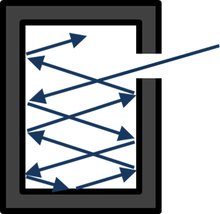
\includegraphics[width=0.2\textwidth]{img/Introduccion/cavidad_cuerpo_negro2.png}
            \caption{Ilustración del cuerpo negro}\label{fig: f1}
        \end{figure}
        
        \vspace{5mm}

        La física clásica es incapaz de explicar la radiación emitida por un cuerpo negro en función de la longitud de onda,
        hasta que la explicación de este fenómeno vino de la mano de \textit{Max Planck} en el siglo \textit{XX}, el cual establece que la energía liberada por el cuerpo negro se emite en pequeños paquetes, llamados \textit{cuantos de energía}. Esta energía es proporcional a una pequeña constante, la constante de Planck, de manera que la energía emitida por el cuerpo negro no es continua, sino que toma un valor discreto que ha de ser múltiplo de dicha constante por su frecuencia de onda, rompiendo completamente con la física de la época y dando el nacimiento a un nuevo campo de la física, la mecánica cuántica.

        \vspace{5mm}

        \begin{equation}
            E = h \nu
            \label{eq: planck}
        \end{equation}

        \vspace{5mm}

        Siendo \( h \) la denominada \textit{constante de Planck}, la cual alcanza un valor de \( 6.62607015 \times 10^{-34} \, \text{J} \cdot \text{s} \), y siendo \( \nu \) la frecuencia. Esta energía o intensidad que libera el cuerpo la podemos medir, en función de su longitud de onda, obteniendo la siguiente gráfica:

        \vspace{5mm}

        \begin{figure}[h]
            \centering
            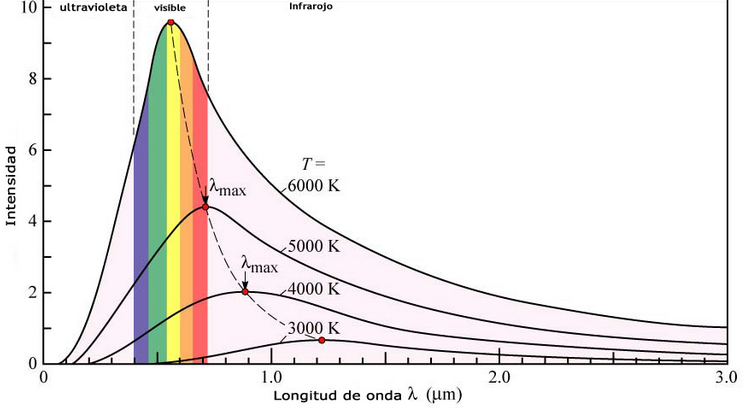
\includegraphics[width=0.75\textwidth]{img/Introduccion/catastrofe_ultravioleta.png}
            \caption{Catástrofe del ultravioleta}
            \label{fig: f2}
        \end{figure}

        \vspace{5mm}

        Podemos observar que a diferentes temperaturas (longitudes de onda) llegamos a diferentes curvas. La física clásica intentaba predecir estas curvas mediante ciertos modelos, que, aunque se ajustaban correctamente en distintas zonas de la gráfica, no se acercaban ni mucho menos a la realidad. Un ejemplo de esto es la catástrofe del ultravioleta, como resultado de no ajustarse correctamente en la zona ultravioleta, en la que la intensidad de la energía tendía a infinito como resultado de otros modelos, en lugar de tender a cero como propuso \textit{Max Planck}, formulando una ecuación que describe perfectamente la figura (\ref{fig: f2}):

        \vspace{5mm}

        \begin{equation}
            B_{\nu}(T) = \frac{2h\nu^3}{c^2} \frac{1}{e^{\frac{h\nu}{k_B T}} - 1}
            \label{eq: planck_ultravioleta}
        \end{equation}

        \vspace{5mm}

        Donde \textit{h} es la \textit{constante de Planck}, \( \nu \) la frecuencia de la radiación, \textit{c} la velocidad de la luz en el vacío, \( k_B \) la \textit{constante de Boltzmann}, \textit{T} la temperatura, y \textit{e} como base de los logaritmos naturales. No obstante, esta teoría cuántica fue primeramente descartada por los físicos de la época, al establecer que la energía no es un valor continuo sino discreto, hasta que con la llegada del efecto fotoeléctrico de \textit{Albert Einstein} todo comenzó a cobrar sentido.

        \vspace{5mm}    

        A finales del siglo XIX, en 1888, se presenta el efecto fotoeléctrico, definido por \textit{Heinrich Hertz}, que consiste en la emision de electrones (fotoelectrones) al incidir luz sobre un metal, actuando como cátodo, los cuales se recogen en un ánodo, generando corriente en un circuito. Dicha luz suele ser ultravioleta, aunque en algunos casos puede ser visible.

        \vspace{5mm}

        Previamente al experimento, se plantearon varias hipótesis en base a la física clásica de la época:

        \begin{itemize}
            \item El aumento de la intensidad de la luz incrementaría la energía cinética de los fotoelectrones emitidos.
            \item A mayor frecuencia mayor intensidad de corriente en el circuito. 
        \end{itemize}

        \vspace{5mm}

        Los resultados de dicho experimento fueron sorprendentes, ya que se observó que la energía cinetica de los electrones que poseen el cátodo no dependen de la intensidad de la luz, sino de su frecuencia, y adicionalmente se pudo ver que a mayor intensidad de luz mayor intensidad de corriente. Más tarde, en 1905, se presentó un artículo, ciertamente atrevido teniendo en cuenta los recursos de la época, que resolvía todos estos problemas.

        \vspace{5mm}

        \textit{Albert Einstein} presentó su hipótesis para el efecto fotoeléctrico, basándose en los resultados del experimento de \textit{Planck}, aclarando que la luz no se comporta como una onda, sino que está compuesta de pequeñas partículas, llamadas \textit{fotones}, cuya energía depende de su frecuencia, como ya propuso \textit{Max Planck} en (\ref{eq: planck}), rompiendo de nuevo con los principios de la física clásica.

        \vspace{5mm}

        En dicha hipótesis se establece la necesidad de una frecuencia mínima, denominada frecuencia umbral, para que el efecto fotoeléctrico tenga lugar, la cual depende del material del que esté construido el cátodo. Por lo que si la frecuencia de los \textit{fotones} emitidos por el haz de luz es menor a esta frecuencia umbral, no se produce corriente en el circuito, por muy intensa que sea la luz. De esta manera, si la frecuencia es mayor o igual a la umbral, los \textit{fotoelectrones} se trasladarán hacia el ánodo al ser expulsados del núcleo de sus átomos, generando energía cinética y por lo tanto, intensidad de corriente en el circuito. Esto lo podemos razonar con la siguiente ecuación:

        \vspace{5mm}

        \begin{equation}
            E_e = E_{ionizacion} + E_{cinetica}
            \label{eq: einstein_fotoelectrico}
        \end{equation}

        \vspace{5mm}

        Esta ecuación tiene sentido visto lo anterior, de manera que la energía de los electrones del cátodo ha de ser igual a su \textit{energía de ionización} (o también conocido como \textit{trabajo de extracción}), la cual es la cantidad de energía necesaria para que se produzca el efecto fotoeléctrico, sumado a su \textit{energía cinética}. Por la explicación vista anteriormente, sabemos que dicha \textit{energía de ionización} depende de la \textit{frecuencia umbral \( \nu_{0} \)}, y con la ecuación de la energía de \textit{Planck} (\ref{eq: planck}), además de conocer la \textit{energía cinética} de una partícula, podemos desarrollar la expresión (\ref{eq: einstein_fotoelectrico}):

        \vspace{5mm}

        \begin{equation*}
            h \nu = h \nu_{0} + \frac{1}{2} m_{e} v_{e}^{2}
        \end{equation*}

        \vspace{5mm}

        Donde \textit{h} es la \textit{constante de Planck}, \( \nu \) es la \textit{frecuencia}, \( \nu_{0} \) es la \textit{frecuencia umbral}, \( m_{e} \) es la masa del electrón, y \( v_{e} \) la velocidad del electrón, en este caso al cuadrado. 
        
        \vspace{5mm}

        Estos son solo dos de los múltiples experimentos con soluciones extrañas para los físicos clásicos de aquella época, en los que, como hemos visto, el comportamiento de ciertos fenómenos, teóricamente imaginados como funciones de onda, se comportan como partículas. También se da el fenómeno contrario, experimentos planteados como partículas pero que son razonados mediante funciones de onda. Esto se definió con el nombre de \textit{dualidad onda-corpúsculo}.
        
        \vspace{5mm}

        Más tarde, tras estudiar a fondo las bases de la mecánica cuántica propuesta por \textit{Max Planck} y \textit{Albert Einstein}, \textit{Louis de Broglie} propuso en su tesis doctoral, en \textit{1924}, que no solo la luz tiene un carácter ondulatorio, sino que toda partícula material, como los electrones, tienen una naturaleza ondulatoria, cuya longitud de onda \( \lambda \) es:
        
        \vspace{5mm}

        \begin{equation}
            \lambda = \frac{h}{p}
            \label{eq: longitud de onda}
        \end{equation}

        \vspace{5mm}

        Donde \textit{p} se refiere al \textit{momento lineal} de la partícula, lo cual podemos expresar como \( p = m \cdot v \), siendo \textit{m} la masa, y \textit{v} la velocidad de la partícula. Tras el razonamiento de \textit{Broglie} en \textit{1924}, surge la \textit{función de onda} en una dimensión, la cual describe el comportamiento las partículas con carácter ondulatorio:

        \vspace{5mm}

        \begin{equation}
            \varphi (x, t) = e^{i(px - Et) / \hbar}
            \label{eq: funcion_de_onda}
        \end{equation}

        \vspace{5mm}

        Siendo \textit{i} la unidad imaginaria, \( \hbar \) la \textit{constante de Planck normalizada}

        \vspace{5mm}

        \begin{equation}
            \hbar = \frac{h}{2\pi} 
            \label{constante_planck_normalizada}
        \end{equation}    

        \vspace{5mm}
        
        y \textit{x} y \textit{t} las coordenadas de posición y tiempo de la partícula. Sin embargo, todavia no se conocia su significado fisico con total exactitud. No fue hasta que con el experimento de la doble rendija de \textit{Clinton Davisson} y \textit{Lester Germer} sobre electrones en \textit{1927} (aunque \textit{Thomas Young} lo propuso en \textit{1801}, sobre un haz de luz, demostrando su naturaleza ondulatoria) que se confirmó la hipótesis de \textit{De Broglie}. Como su propio nombre indica, dicho experimento consiste en una superficie opaca con dos rendijas, detrás de la cual colocamos un detector de partículas para poder percibir el comportamiento de los electrones o fotones que pasan a través de ambas rendijas. Según la física clásica, se espera que las partículas pasen a través de las rendijas en forma de línea recta, como lo haría cualquier objeto. Sin embargo, esto no sucede así en el contexto de la mecánica cuántica.

        \vspace{5mm}

        \begin{figure}[h]
            \centering
            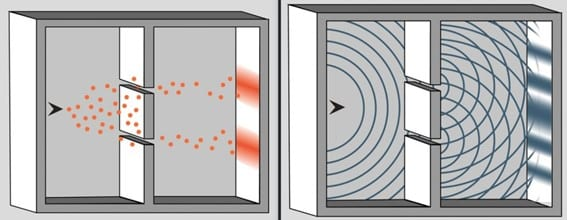
\includegraphics[width=0.75\textwidth]{img/Introduccion/doble_rendija.png}
            \caption{Experimento de la doble rendija}
            \label{fig: doble_rendija}
        \end{figure}

        \vspace{5mm}

        Al realizar el experimento, podemos observar un patrón de interferencias en la pantalla de detección situada detrás de las rendijas, el cual es muy similar al patrón que siguen las ondas cuando se superponen unas con otras. Efectivamente, las ondas asociadas a cada partícula se superponen unas con otras como se reveló en el experimento, no obstante, cuando observamos estas partículas mediante el detector, se comportan como una partícula clásica, cambiando su comportamiento, de manera que podemos ver por qué rendija cruzó la partícula. Este fenómeno se conoce como \textit{colapso de función de onda}, y existen muchas teorías que intentar explicar esto, siendo la más famosa la \textit{intepretación de Copenhage}, en la que se establece que la observación de la partícula produce un colapso de su función de onda, determinando su estado correspondiente a la medición.

        \vspace{5mm}

        Matemáticamente, podemos expresar la superposición de ondas como una superposición de estados, esto es:

        \vspace{5mm}

        \begin{equation}
            \psi(x, t) = \psi_{1}(x, t) + \psi_{2}(x, t) + \dots + \psi_{n}(x, t), \qquad \forall n \in \mathbb{N} \setminus \{0\}
            \label{eq: superposicion}
        \end{equation}

        \vspace{5mm}

        Adicionalmente, surgieron ciertas dudas relacionadas con la naturaleza de la función de onda. Es lógico preguntarse que, si las partículas están definidas por funciones de onda, ¿Dónde están realmente las partículas? Ya que una partícula no puede estar en varios puntos a la vez, ha de estar en un único punto. Es aquí cuando entró \textit{Max Born}, quien sugiere que \( \lvert \psi(x, t) \rvert ^ {2} \) no es simplemente el cuadrado del módulo de la función de onda, sino que es una función de densidad de probabilidad, de manera que, para cada instante de tiempo y una región del espacio, la siguiente integral

        \vspace{5mm}

        \begin{equation}
            \int_{E} \lvert \psi(x, t) \rvert ^ {2} dx, \qquad \forall t \in \mathbb{R}, E \subset \Omega
            \label{eq: densidad_probabilidad_onda}
        \end{equation}

        \vspace{5mm}

        Representa la densidad de probabilidad de encontrar una partícula para un valor de \textit{t} en una determinada región \textit{E} del espacio \( \Omega \), de manera que podemos deducir una condición que ha de cumplir la expresión (\ref{eq: densidad_probabilidad_onda}):
        
        \vspace{5mm}

        \begin{equation}
            \int_{\Omega} \lvert \psi(x, t) \rvert ^ {2} dx = 1, \qquad \forall t \in \mathbb{R}
            \label{eq: interpretacion_probabilistica}
        \end{equation}

        \vspace{5mm}
        
        Esto tuvo una importancia bastante profunda en la mecánica cuántica de la época y en la física en general, ya que las únicas ideas de probabilidad estaban relacionadas a sistemas de incertidumbre, como el lanzamiento de una moneda. De esta manera se concluyó en la probabilidad como uno de los principales focos de la física y de la comprensión de las partículas subatómicas.

        \vspace{5mm}

        Esto concluye, al no poder medir con exactitud el estado de una partícula, como ocurre en la física clásica, en el \textit{principio de incertidumbre} de \textit{Heisenberg} en \textit{1927}, estableciéndose que en la medición de una partícula no podemos conocer con completa exactitud la posición y el momento lineal a la vez, sino que cuanto más preciso midamos su posición exacta menos precisa será la medición del momento lineal de dicha partícula y viceversa.

    \vspace{5mm}





    \newpage
    \thispagestyle{empty}
    \mbox{}

    \section{La Ecuación de Schrödinguer}\label{sec: la_ecuacion_de_schrodinguer}

    \subsection{Obtención de la Ecuación de Schrödinguer}

    \vspace{5mm}

    Todas las ideas vistas anteriormente, la función de onda (\ref{eq: funcion_de_onda}), la superposición cuántica (\ref{eq: superposicion}) y la interpretacion probabilística de la función de onda (\ref{eq: densidad_probabilidad_onda}) dieron lugar a la necesidad de decribir la evolución de la función de onda \( \psi(x, t) \) en función del tiempo \textit{t}. Es en este momento cuando aparece \textit{Erwin Schrödinguer} en \textit{1926}, presentando su famosa ecuación, obtenida de derivar y desarrollar la ecuación  (\ref{eq: funcion_de_onda}). 
    
    En primer lugar, derivamos (\ref{eq: funcion_de_onda}) con respecto al tiempo \textit{t}:
    \begin{align*}
        \frac{\partial}{\partial t} \psi(x, t) &= \frac{\partial}{\partial t} e^{i(px - Et) / \hbar} \\[8pt]
        \frac{\partial}{\partial t} \psi(x, t) &= e^{i(px - Et) / \hbar} \left(- \frac{iE}{\hbar} \right)
    \end{align*}
    Podemos observar que vuelve a aparecer la función de onda (\ref{eq: funcion_de_onda}), al tratarse de una función exponencial:
    \begin{equation*}
        \frac{\partial}{\partial t} \psi(x, t) = - \frac{iE}{\hbar} \psi(x, t)
    \end{equation*}
    A continuación multiplicamos ambos miembros por \( i\hbar \), para eliminar los denominadores y substrayendos de la expresión:
    \begin{equation}
        i \hbar \frac{\partial}{\partial t} \psi(x, t) = E \psi(x, t)
        \label{eq: obtencion_schrodinguer}
    \end{equation}
    Esta expresión la reservaremos para más adelante, ya que, en los siguientes cálculos, necesitaremos el producto de la energía del sistema \( E \) y la función de onda \( \psi \). Como siguiente paso, vamos a continuar derivando la función de onda (\ref{eq: funcion_de_onda}) con respecto de \textit{x}:
    \begin{align*}
        \frac{\partial}{\partial x} \psi(x, t) &= \frac{\partial}{\partial x} e^{i(px - Et) / \hbar} \\[10pt]
        \frac{\partial}{\partial x} \psi(x, t) &= e^{i(px - Et) / \hbar} \left( \frac{ip}{\hbar} \right) \\[10pt]
        \frac{\partial}{\partial x} \psi(x, t) &= \frac{ip}{\hbar} \psi(x, t)
    \end{align*}
    Derivamos por segunda vez respecto de la variable espacial:
    \begin{align*}
        \frac{\partial}{\partial x^{2}} \psi(x, t) &= \frac{\partial}{\partial x} \left( \frac{ip}{\hbar} \psi(x, t) \right) \\[10pt]
        \frac{\partial}{\partial x^{2}} \psi(x, t) &= - \frac{p^{2}}{\hbar^{2}} \psi(x, t)
    \end{align*}
    Multiplicamos por (\( - \frac{\hbar^{2}}{2m} \)) para obtener lo siguiente:
    \begin{equation*}
        - \frac{\hbar^{2}}{2m} \frac{\partial}{\partial x^{2}} \psi(x, t) = \frac{p^{2}}{2m} \psi(x, t)
        \\[2mm]
    \end{equation*}
    Conociéndose que la energía cinética es \( E = \frac{p^{2}}{2m} \), obtenemos la siguiente expresión
    \begin{equation*}
        - \frac{\hbar^{2}}{2m} \frac{\partial}{\partial x^{2}} \psi(x, t) = E \psi(x, t)
    \end{equation*}
    Sustituyendo el valor que acabamos de obtener \( E \psi(x, t) \) en (\ref{eq: obtencion_schrodinguer}), llegamos prácticamente a la ecuación que estamos buscando:
    \begin{equation*}
        i \hbar \frac{\partial}{\partial t} \psi(x, t) = - \frac{\hbar^{2}}{2m} \frac{\partial}{\partial x^{2}} \psi(x, t)
        \\[2mm]
    \end{equation*}
    Para terminar, si agregamos la energía potencial y generalizamos la ecuación para más de una dimensión espacial, obtenemos la famosa \textbf{\textit{ecuación de Schrödinguer}}:
    \begin{equation}
        \boxed{i \hbar \frac{\partial}{\partial t} \psi(x, t) = (- \frac{\hbar^{2}}{2m} \Delta + V(x, t)) \psi(x, t)} 
        \label{eq: ecuacion_schrodinguer}     
    \end{equation}
    Siendo \( \Delta \) el operador Laplaciano en coordenadas canónicas, que se define como
    \begin{equation*}
        \Delta = \frac{\partial}{\partial^{2} x_{1}} + \cdots + \frac{\partial}{\partial^{2} x_{n}}, \qquad \forall n \in \mathbb{N}
    \end{equation*}

    \vspace{5mm}





    \subsection{La Ecuación de Schrödinguer Independiente del Tiempo}

    \vspace{5mm}

    A continuación, para obtener la \textit{ecuación de Schrödinguer independiente del tiempo} tenemos que plantearnos obtener las soluciones de la ecuación de Schrödinguer (\ref{eq: ecuacion_schrodinguer}). Para simplificar cálculos, vamos a suponer que la energía potencial \( V(x) \) en (\ref{eq: ecuacion_schrodinguer}) depende única y exclusivamente de la variable espacial \textit{x}, de manera que podemos probar a encontrar soluciones por el método de \textit{separación de variables}. Supongamos una solución como producto de dos funciones \( \psi(x) \) y \( \tau(t) \):

    \begin{equation*}
        \Psi(x, t) = \psi(x) \tau(t) \\[5pt]
    \end{equation*}

    Sustituyendo en (\ref{eq: ecuacion_schrodinguer}) nos queda como

    \begin{equation*}
        i \hbar \frac{\partial}{\partial t} \psi(x) \tau(t) = \left( - \frac{\hbar^{2}}{2m} \Delta + V(x) \right) \psi(x) \tau(t) \\[5pt]
    \end{equation*}

    Podemos dividir entre \( \psi(x) \tau(t) \) y ordenar ambos miembros, de manera que un miembro nos quede únicamente en función de \textit{x} y otro en función de \textit{t}:

    \begin{equation*}
        i \hbar \frac{1}{\tau(t)} \frac{\partial}{\partial t} \tau(t) = V(x) - \frac{\hbar^{2}}{2m} \frac{1}{\psi(x)} \frac{\partial}{\partial x^{2}} \psi(x) \\[5pt]
    \end{equation*}

    Hemos de recalcar que hemos tomado el laplaciano \( \Delta \) como \( \frac{\partial}{\partial x^{2}} \), siendo este el laplaciano en una dimensión espacial, con el fin de simplificar los cálculos. Llegados a este punto, para que se cumpla la igualdad, cada miembro de la ecuación ha de ser igual a una constante \( E \), al demostrarse que se trata de una ecuación separable
    
    \begin{equation}
        \begin{cases}
            \displaystyle i \hbar \frac{1}{\tau(t)} \frac{\partial}{\partial t} \tau(t) = E \\[10pt]
            \displaystyle V(x) - \frac{\hbar^{2}}{2m} \frac{1}{\psi(x)} \frac{\partial}{\partial x^{2}} \psi(x) = E \\[10pt]
        \end{cases}
        \label{eq: separacion_variables}
    \end{equation}

    Tomando como base la primera ecuación del sistema, podemos obtener una solución exponencial de la siguiente manera:
        
    \begin{align*}
        \frac{\partial}{\partial t} \tau(t) &= \frac{E}{i \hbar} \tau(t) \\[10pt]
        \tau(t) &= e ^ { \left( - \frac{Ei}{\hbar} \right) t}
    \end{align*}

    Esto nos proporciona una evolución temporal del sistema en el que se encuentra la partícula. Sin embargo, para obtener la ecuación que estamos buscando, hemos de fijarnos en la segunda ecuación de (\ref{eq: separacion_variables}):

    \begin{equation*}
        V(x) - \frac{\hbar^{2}}{2m} \frac{1}{\psi(x)} \frac{\partial}{\partial x^{2}} \psi(x) = E
    \end{equation*}

    La cual podemos reescribir como

    \begin{equation}
        \left( - \frac{\hbar^{2}}{2m} \frac{\partial}{\partial x^{2}} + V(x) \right) \psi(x) = E \psi(x) \\[5pt]
        \label{eq: schrodinguer_independiente_tiempo}
    \end{equation}

    En muchas referencias, la ecuación (\ref{eq: schrodinguer_independiente_tiempo}) es ya la ecuación que estamos buscando. Sin embargo, nosotros la vamos a denotar en función del operador \textit{Hamiltoniano} \( H \), el cual representa la energía total de nuestro sistema cuando ésta permanece constante en el tiempo, que en nuestro caso sucede al establecer que \( V(x, t) = V(x) \). Así, la \textbf{\textit{ecuación de Schrödinguer independiente del tiempo}} queda como
    
    \begin{equation}
        \boxed{ H \psi(x) = E \psi(x)}
        \label{eq: schrodinguer_independiente_tiempo_hamiltoniano}
    \end{equation}

    Siendo \( H = \left( - \frac{\hbar^{2}}{2m} \frac{\partial}{\partial x^{2}} + V(x) \right) \) el operador \textit{Hamiltoniano}. Finalmente, podemos concluir que la solución completa queda como

    \begin{equation}
        \Psi(x, t) = e ^ { \left( - \frac{Ei}{\hbar} \right) t} \psi(x)
    \end{equation}

    \vspace{5mm}

    La ecuación (\ref{eq: schrodinguer_independiente_tiempo_hamiltoniano}) describe los estados estacionarios de una partícula en el potencial \( V(x) \) y es usada en muchos sistemas físicos de vital importancia (generalmente aquellos cuyo potencial no depende del tiempo \( t \)) como átomos y moléculas en estado estacionario, siempre y cuando el sistema se encuentre en equilibrio y no haya fuerzas externas que varíen el valor de la energía potencial con respecto al tiempo, pozos de potencial infinito, osciladores armónicos, o campos eléctricos y gravitacionales constantes.

    \vspace{5mm}

    Sin embargo, hay otras muchas situaciones en las que el potencial no solo depende de la posición \( x \), de manera que no podemos aplicar el método de separación de variables visto anteriormente, como partículas en campos magnéticos, problemas asociados a la relatividad, o sistemas caóticos. Para estos sistemas utilizamos otros métodos de resolución, como simulaciones numéricas, para alcanzar la solución del sistema.

    \vspace{5mm}


    


    \newpage
    \thispagestyle{empty}
    \mbox{}

    \section{El Espacio de Hilbert}\label{sec: el_espacio_de_Hilbert}

    \vspace{5mm}

    En el contexto de la mecánica cuántica, el \textit{espacio de Hilbert}, el cual denotaremos como \( \mathcal{H} \), es el marco matemático en el que nos apoyamos para explicar el estado físico de las partículas subatómicas, como ya veremos en la sección (\ref{sec: postulados}) explicando los postulados. Este \textit{espacio de Hilbert} es simplemente una generalización de los espacios euclídeos \( \mathbb{R}^{n} \) sobre el cuerpo de los números reales \( \mathbbl{R} \) o sobre los números complejos \( \mathbb{C} \), siendo en el caso de la mecánica cuántica, como podremos imaginar, una generalización sobre \( \mathbb{C} \) ya que la geometría compleja juega un papel fundamental en este campo de la física.
    
    \vspace{5mm}

    Una vez hemos introducido los \textit{espacios de Hilbert}, vamos a pasar a explicar sus propiedades básicas, para poder comprender los conceptos que vendrán más adelante en los siguientes capítulos. La diferencia fundamental con respecto a los espacios euclídeos \( \mathbb{R}^{n} \), además de que las distintas componentes de los vectores \( \ket{\psi} \in \mathcal{H} \) son complejas, reside en el producto escalar, el cual para un espacio euclídeo \( \mathbb{R}^{n} \) podemos expresar de la siguiente manera

    \begin{equation*}
        \braket{v, w} = \sum_{i = 0}^{N - 1} v_{i} w_{i}, \qquad \forall \ v_{i}, w_{i} \in \mathbb{R}^{n}
    \end{equation*}

    \vspace{2.5mm}

    Siendo \( N \) la dimensión del espacio euclídeo \( \mathbb{R}^{n} \). La principal diferencia es que un \textit{espacio de Hilbert} \( \mathcal{H} \) cuenta con un producto escalar hermítico, el cual definiremos a continuación.

    \vspace{5mm}

    Consideremos un espacio vectorial \( \mathcal{H} = \{ \ket{\psi}, \ket{\phi}, \cdots \} \) sobre el cuerpo de los números complejos \( \mathbb{C} \), de manera que se cumplen la propiedad de la suma y la multiplicación por un escalar:
    \begin{align*}
        \ket{\psi} + \ket{\phi} \in \mathcal{H}, \qquad &\forall \ket{\psi}, \ket{\phi} \in \mathcal{H}\\[10pt]
        \alpha \ket{\psi} \in \mathcal{H}, \qquad &\forall \ket{\psi} \in \mathcal{H} \quad \text{y} \quad \forall \alpha \in \mathbb{C}
    \end{align*}

    \vspace{1.5mm}

    Además, dicho espacio vectorial \( \mathcal{H} \) cuenta con un producto escalar hermítico, el cual es una aplicación
    \begin{align*}
        \mathcal{H} \times \mathcal{H} &\longrightarrow \mathbb{C} \\
        \ket{\phi}, \ket{\psi} &\longrightarrow \braket{\phi \ | \ \psi}
    \end{align*}

    \vspace{1.5mm}

    Que cumple con las propiedades de linealidad y hermiticidad, respectivamente:
    \begin{align*}
        \braket{\phi \ | \ \lambda_{1}\psi_{1} + \lambda_{2}\psi_{2}} &= \lambda_{1} \braket{\phi \ | \ \psi_{1}} + \lambda_{2} \braket{\phi \ | \ \psi_{2}}, \qquad \forall \lambda_{1}, \lambda{2} \in \mathbb{C} \\[10pt]
        \braket{\phi \ | \ \psi} &= \braket{\psi \ | \ \phi}^{*}
    \end{align*}

    \vspace{1.5mm}

    Siendo \( \braket{\psi \ | \ \phi}^{*} \) la expresión conjugada compleja de \( \braket{\phi \ | \ \psi} \). Esta aplicación ha de ser definida positiva, de manera que
    \begin{equation*}
        \braket{\psi \ | \ \psi} \geq 0 \quad \text{y} \quad \braket{\psi \ | \ \psi} = 0 \ \Leftrightarrow \ \ket{\psi} = 0
    \end{equation*}

    \vspace{1.5mm}

    Si \( \mathcal{H} \) satisface estas propiedades, podemos concluir que \( \mathcal{H} \) es un espacio de Hilbert. Con esto podemos definir la norma de un vector \( \psi \) como
    \begin{equation}
        \| \psi \| = \sqrt{\braket{\psi \ | \ \psi}} \qquad \in \mathbb{R} \geq 0
        \label{eq: norma_producto_escalar}
    \end{equation}

    \vspace{1.5mm}

    Podemos observar que \( \| \psi \| \in \mathbb{R} \geq 0 \), ya que al tratarse de la longitud de un vector, ha de ser un número real no negativo. Con esto podemos introducir la desigualdad de Schwartz, la cual establece lo siguiente:
    \begin{equation}
        \| \braket{\phi \ | \ \psi} \| ^{2} \leq \| \phi \| ^{2} \| \psi \|^{2}
        \label{eq: desigualdad_schwartz}
    \end{equation}

    \vspace{1.5mm}

    Al complirse esta expresión, el producto interno está bien definido, de donde obtenemos la norma como ya vimos en (\ref{eq: norma_producto_escalar}), pasando a ser un espacio normado cuya norma cumple con la \textit{sucesión de Cauchy}:
    \begin{equation*}
        \forall \epsilon > 0, \quad \exists N \in \mathbb{N} \ \text{tal que} \ m, n \geq N \implies \| x_{n} - x_{m} \| < \epsilon
    \end{equation*}
    
    \vspace{1.5mm}

    por lo que además es un espacio completo.

    \vspace{5mm}

    Con esto ya podemos llegar a la conclusión de que, un espacio de Hilbert, en resumidas cuentas, es un espacio vectorial \( \mathcal{H} \) con un producto escalar hermítico, y por lo tanto sobre el cuerpo de los números complejos \( \mathbb{C} \). Aún así, vamos a profundizar más en la definición de \textit{producto escalar hermítico} en \( \mathcal{H} \). Para ello, vamos a trabajar sobre el concepto de \textit{espacio dual} y \textit{ortonormalidad} definiendo una base ortonormal de nuestro espacio vectorial \( \mathcal{H} \), como
    \begin{equation}
        B = \{ \ket{e_{j}} \} _{j = 0}^{N - 1}
        \label{eq: base_ortonormal_H}
    \end{equation}

    \vspace{1.5mm}

    Donde \( N \) es la dimensión de \( \mathcal{H} \). No obstante, esto no deja de ser una base común y corriente. Para que esta base sea ortonormal, se tienen que dar las condiciones de ortonormalidad, en las que se establece que el producto escalar de dos vectores distintos de dicha base es cero, y la norma de ambos vectores ha de ser igual a la unidad. Esto lo podemos formalizar de la siguiente manera
    \begin{align}
        \braket{e_{1} | e_{2}} = \delta_{e_{1}, e_{2}}, \qquad &\forall \ \ket{e_{1}}, \ket{e_{2}} \in B \label{eq: ortonormalidad} \\
        \| e_{j} \| = 1,  \qquad &\forall \ \ket{e_{j}} \in B \label{eq: linealidad}
    \end{align}
    
    \vspace{1.5mm}

    Donde \( \delta_{n, m} \) en (\ref{eq: ortonormalidad}) es la función \textit{delta de Kronecker}, que se define como
    \begin{equation}
        \delta_{i, j} = 
        \begin{cases}
            1, & \text{si } i = j, \\
            0, & \text{si } i \neq j
        \end{cases}
        \label{eq: delta_kronecker}
    \end{equation}

    \vspace{1.5mm}

    Así, el producto escalar de dos vectores de una base ortonormal siempre va a ser cero, y el producto escalar de un vector cualquiera \( \ket{\psi} \in \mathcal{H} \) consigo mismo es la unidad
    \begin{align}
        \braket{e_{1} | e_{2}} = 0, &\qquad \forall \ e_{1}, e_{2} \in B \\[10pt]
        \| \psi \| = \sqrt{\braket{\psi \ | \ \psi}} = 1, &\qquad \forall \ \ket{\psi} \in \mathcal{H}
    \end{align}

    \vspace{1.5mm}

    Entonces, podemos expresar cualquier vector de nuestro espacio vectorial \( \mathcal{H} \) como una combinación lineal de los vectores de la base:
    \begin{equation}
        \ket{\psi} = \sum_{j = 0}^{N - 1} c_{j} \ket{e_{j}}, \qquad \forall \ \ket{\psi} \in \mathcal{H} \quad \text{y} \quad \ \forall c_{j} \in \mathbb{C}
        \label{eq: combinacion_lineal_Hilbert}
    \end{equation}

    \vspace{1.5mm}

    Esto es muy importante ya que vamos a usar estos vectores para ver el estado en el que se encuentra nuestro sistema cuantico. Esto está directamente ligado con la superposición de la función de onda, como ya vimos en (\ref{eq: superposicion}), ya que, cada uno de los posibles estados de una partícula en una superposición de funciones de onda, no son más que los vectores de una base ortonormal perteneciente a un espacio de Hilbert \( \mathcal{H} \). Esto es de vital importancia y lo seguiremos viendo cuando introduzcamos los estados de un \textit{qubit}, como ya veremos más adelante.

    \vspace{5mm}

    Ahora vamos a dar las primeras nociones del \textit{espacio dual} \( \mathcal{H} ^ {*} \) de \( \mathcal{H} \). Si tenemos un espacio de Hilbert \( \mathcal{H} \) sobre el cuerpo de los número complejos \( \mathbb{C} \), definimos su \textit{espacio dual} \( \mathcal{H} ^ {*} \) como el conjunto de todas las aplicaciones lineales que transforman elementos de \( \mathcal{H} \), es decir, \textit{kets}, en un número complejo \( \mathbb{C} \)
    \begin{equation*}
        \mathcal{H} ^ {*} = \{ \bra{\phi}: \mathcal{H} \longrightarrow \mathbb{C} \}
    \end{equation*}

    \vspace{1.5mm}

    Donde \( \bra{\phi} \) se construye con el conjugado hermítico, el cual se define con el operador \( \dagger \):
    \begin{equation}
        ( \ket{\phi} )^{\dagger} = \bra{\phi}
        \label{eq: conjugado_hermitico}
    \end{equation}

    \vspace{1.5mm}

    Aprovechamos para explicar la notación, en la tenemos los elementos pertenecientes al espacio dual \( \mathcal{H} ^ {*} \) conocidos como \textit{bra} \( \bra{\phi} \), vectores pertenecientes al espacio de Hilbert \( \mathcal{H} \) que son llamados como \textit{kets} \( \ket{\psi} \), y el resultado de aplicar un producto escalar hermítico sobre un \textit{bra} y un \textit{ket}, al que haremos referencia como \textit{bracket} \( \braket{\phi \ | \ \psi} \).

    \vspace{5mm}

    El espacio dual \( \mathcal{H} ^ {*} \) tiene una base dual asociada
    \begin{equation}
        B ^ {*} = \{ \bra{e_{i}} \} _{i = 0}^{N - 1}
    \end{equation}

    \vspace{1.5mm}

    mediante la que, de la misma manera que con la base \( B \) definida en (\ref{eq: base_ortonormal_H}) sobre un espacio de Hilbert \( \mathcal{H} \), podemos expresar cualquier \textit{bra} \( \bra{\phi} \in \mathcal{H} ^ {*} \) como una combinación lineal de los \textit{bra} de la base \( B ^ {*} \):
    \begin{equation}
        \bra{\phi} = \sum_{i = 0}^{N - 1} d_{i}^{*} \bra{e_{i}}, \qquad \forall \ \bra{\phi} \in B^{*} \quad y \quad \forall \ c_{i}^{*} \in \mathbb{C}
        \label{eq: combinacion_lineal_hilbert_dual}
    \end{equation}    

    \vspace{1.5mm}

    Por lo tanto, la actuación de un \textit{bra} \( \bra{\phi} \in \mathcal{H}^{*} \) sobre un \textit{ket} \( \ket{\psi} \in \mathcal{H} \) es el producto escalar hermítico de los \textit{kets}, y debido a la propiedad de linealidad en \( \mathcal{H} \), este producto queda perfectamente definido en \( \mathcal{H} \)
    \begin{equation*}
        \braket{\phi \ | \ \psi} = \ket{\phi} \cdot \ket{\psi} = \left( \sum_{i = 0}^{N - 1} d_{i}^{*} \bra{e_{i}} \right) \left( \sum_{j = 0}^{N - 1} c_{j} \ket{e_{j}} \right) = \sum_{i = 0}^{N - 1} \sum_{j = 0}^{N - 1} d_{i}^{*} \ c_{j} \ \braket{e_{i} \ | \ e_{j}} = \sum_{i = 0}^{N - 1} \sum_{j = 0}^{N - 1} d_{i}^{*} \ c_{j} \ \delta_{e_{i}, e_{j}} = \sum_{i = 0}^{N - 1} d_{i}^{*} \ c_{i}
    \end{equation*}
    \begin{equation}
        \boxed{\braket{\phi \ | \ \psi} = \sum_{i = 0}^{N - 1} d_{i}^{*} \ c_{i}}
        \label{eq: producto_escalar_desarrollado}
    \end{equation}

    \vspace{1.5mm}

    Por lo que, el producto escalar hermítico \( \braket{\phi \ | \ \psi} \) es simplemente multiplicar los complejos conjugados \( d_{i}^{*} \) provenientes del \textit{bra} \( \bra{\phi} \) por los distintos elementos \( c_{i} \) de los vectores \( \ket{\psi} \) del espacio de Hilbert \( \mathcal{H} \). 

    \vspace{5mm}

    Encontrándonos en este punto, a partir de (\ref{eq: producto_escalar_desarrollado}) podemos desarrollar la norma de un vector en \( \mathcal{H} \), obteniendo que
    \begin{equation}
        \| \psi \| ^{2} = \braket{\psi \ | \ \psi} = \sum_{i = 0}^{N - 1} d_{i}^{*} c_{i} = \sum_{i = 0}^{N - 1} | c_{i} | ^{2} = 1, \qquad \forall \psi \in \mathcal{H}
        \label{eq: norma_vector_hilbert}
    \end{equation}

    \vspace{2.5mm}

    Esto es de vital importancia y nos ayudará a comprender y explicar los \textit{postulados de la mecánica cuántica}, como vamos a ver a continuación.


    \vspace{5mm}

    \subsection{Postulados de la Mecánica Cuántica}\label{sec: postulados}

    \vspace{5mm}

    Una vez hemos asentado las bases históricas de la mecánica cuántica, introducido las funciones de onda, la ecuación de Schrödinguer, y hemos podido apreciar la relación de este campo de la física con el álgebra lineal, por medio de los espacios de Hilbert, estamos en condiciones de enunciar y comprender los postulados de la mecánica cuántica. Estos se podrían definir, a modo de resumen, en los principios fundamentales sobre los que se basa esta nueva teoría para definir el comportamiento de las partículas subatómicas, basándose en resultados experimentales como algunos que ya vimos en la introducción histórica (\ref{sec: historia}). Comencemos por el primer postulado:
    
    \vspace{7.5mm}

    \textbf{Postulado 1}: \textit{Para un instante \( t_{0} \), el estado de un sistema cuántico se puede describir mediante un vector \( \ket{\varphi(t_{0})} \) de un espacio de Hilbert \( \mathcal{H} \)}.

    \vspace{2.5mm}

    Efectivamente, esto es uno de los puntos clave que vimos en (\ref{eq: combinacion_lineal_Hilbert}) tratando sobre el espacio de Hilbert \( \mathcal{H}\), en el que establecíamos que cualquier vector perteneciente a \( \mathcal{H} \), se puede expresar como una combinación lineal de los vectores de la base, siendo esta base ortonormal.

    \vspace{10mm}

    \textbf{Postulado 2}: \textit{Toda magnitud física medible \( \mathcal{A} \) se representa mediante un operador
    hermítico A que actúa sobre \( \mathcal{H} \). Este operador es un observable}.
    
    \vspace{5mm}

    En mecánica cuántica, a las magnitudes se les asigna un operador en concreto, un \textit{observable}, y este \textit{observable} no es más que un operador lineal hermítico. Vamos a ir desglosando punto por punto para enteder todo de la mejor manera posible.

    \vspace{5mm}

    Un operador es un objeto que actúa sobre los elementos de un espacio vectorial, en nuestro caso, un espacio de Hilbert \( \mathcal{H} \), transformándolos en otro vector perteneciente al mismo espacio
    \begin{equation}
        \hat{A} \ket{\psi} \overset{\hat{A}}{\longrightarrow} \ket{\psi '}, \qquad \ket{\psi}, \ket{\psi '} \in \mathcal{H}
        \label{eq: operador_espacio_hilbert}
    \end{equation}

    \vspace{1.5mm}

    Pongamos como ejemplo el producto externo \( \ket{\phi} \bra{\psi} \) multiplicado a un vector \( \ket{\varphi} \in \mathcal{H} \), esto es:
    \begin{equation*}
        \left( \ket{\phi} \bra{\psi} \right) \left( \ket{\varphi} \right) = \ket{\phi} \braket{\psi \ | \ \varphi} = \ket{\phi} k = k \ket{\phi}, \qquad k \in \mathbb{C}
    \end{equation*}

    \vspace{1.5mm}

    Con esto hemos probado que \( \ket{\phi} \bra{\psi} \) es un \textit{operador}, ya que 
    \begin{equation}
        \hat{A} \ket\varphi = k \ket{\phi}, \qquad k \in \mathbb{C}
    \end{equation}

    \vspace{1.5mm}

    Esto resulta en que un operador fruto de un producto externo se puede expresar como una combinación lineal de productos externos de vectores de la base
    \begin{equation}
        \hat{A} = \sum_{i = 0}^{N - 1} \sum_{j = 0}^{N - 1} A_{ij} \ket{i} \bra{j}, \qquad \forall \ \ket{i}, \ket{j} \in B
        \label{eq: operador_combinacion_lineal}
    \end{equation}

    \vspace{1.5mm}

    Podemos ver fácilmente que estos operadores se pueden representar como matrices cuadradas de dimensión \( N \times N \). Además, partiendo de la expresión anterior, existe una condición suficiente y necesaria para que un conjunto de vectores sea base. Esta condición se denomina \textit{relación de cierre}, y se obtiene de particularizar la expresión (\ref{eq: operador_combinacion_lineal}) para el operador identidad \( I \), el cual se define como 
    \begin{equation}
        I_{ij} =
        \left\{
        \begin{array}{ll}
            1, & \text{si } i = j \\
            0, & \text{si } i \neq j
        \end{array}
        \right\}
        = \delta_{ij}
    \end{equation}

    \vspace{1.5mm}

    Entonces, esta relación establece que, si la suma de los \textit{ketbras} \( \ket{i} \bra{j} \) de los elementos de la base es igual al operador identidad \( I \), todos los elementos de dicha base pueden generar el espacio de Hilbert \( \mathcal{H} \), de la siguiente manera
    \begin{align*}
        I &= \sum_{i = 0}^{N - 1} \sum_{j = 0}^{N -1} \delta_{ij} \ket{i} \bra{j} = \sum_{i = 0}^{N -1} \ket{i} \bra{i} \\[10pt]
        I \ket{\psi} &= \sum_{i = 0}^{N - 1} \ket{i} \braket{i \ | \ \psi} = \sum_{i = 0}^{N - 1} c_{i} \ket{i} = \ket{\psi} \\[10pt]
    \end{align*}
    \begin{equation}
        I \ket{\psi} = \psi
        \label{eq: operador_identidad}
    \end{equation}

    \vspace{1.5mm}

    De donde hemos obtenido que \( \braket{i \ | \ \psi} = c_{i} \). Esto lo podemos obtener a partir de (\ref{eq: combinacion_lineal_Hilbert}), de manera que
    \begin{align}
        \braket{i \ | \ \psi} &= \sum_{j = 0}^{N - 1} c_{j} \braket{i \ | \ j} \\[10pt]
        \braket{i \ | \ \psi} &= \sum_{j = 0}^{N - 1} c_{j} \delta_{ij} = c_{i}\label{eq: ci}
    \end{align}
    
    \vspace{1.5mm}

    El resultado que acabamos de obtener en (\ref{eq: ci}), \( c_{i} \), por definición, es la proyección del vector \( \ket{\psi} \in \mathcal{H} \) sobre el vector \( \ket{i} \) de la base. Así, podemos observar que (\ref{eq: operador_identidad}) es efectivamente la identidad \( I \), y que dejará al vector \( \ket{\psi}\) exactamente igual, cumpliéndose así la \textit{relación de cierre}. A continuación, el concepto de linealidad en un operador no es más que
    \begin{equation}
        \hat{A} \left( a \ket{\psi} + b \ket{\phi} \right) = a \hat{A} \ket{\psi} + b \hat{A} \ket{\phi}, \qquad \psi, \phi \in  \mathcal{H} \ \text{y} \ \forall \ a,b \in \mathbb{C} 
        \label{eq: linealidad_operador}
    \end{equation}

    \vspace{1.5mm}

    Y, finalmente, nos queda definir la condición de hermiticidad en un operador, resultando en un \textit{operador hermítico} que, como podemos imaginar, cumple con
    \begin{equation}
        \hat{A} ^ {\dagger} = \hat{A}
        \label{eq: hermiticidad_operador}
    \end{equation}

    \vspace{1.5mm}

    De manera que tras aplicar el operador \( \dagger \) sobre \( \hat{A} \), se vuelve a obtener \( \hat{A} \). Esto conlleva a otra condición, que se obtiene como resultado de (\ref{eq: hermiticidad_operador}):
    \begin{equation*}
        \hat{A} ^ {\dagger} = \sum_{i = 0}^{N - 1} \sum_{j = 0}^{N - 1} A_{ij}^{\dagger} \left( \ket{i} \bra{j} \right) ^ {\dagger} = \sum_{i = 0}^{N - 1} \sum_{j = 0}^{N - 1} A_{ij}^{*} \ket{j} \bra{i} = \sum_{i = 0}^{N - 1} \sum_{j = 0}^{N - 1} A_{ji}^{*} \ket{i} \bra{j}
    \end{equation*}

    \vspace{1.5mm}

    Entonces, como vimos en (\ref{eq: hermiticidad_operador}), para que un operador sea hermítico, su traspuesto conjugado \( \hat{A}^{\dagger} \) ha de ser igual a él mismo \( \hat{A} \), resultando en la siguiente condición
    \begin{align}
        \sum_{i = 0}^{N - 1} \sum_{j = 0}^{N - 1} A_{ji}^{*} \ket{i} \bra{j} &= \sum_{i = 0}^{N - 1} \sum_{j = 0}^{N - 1} A_{ij} \ket{i} \bra{j} \\[10pt]
        A_{ji}^{*} &= A_{ij} \label{eq: hermiticidad_componentes_operador}
    \end{align}

    \vspace{1.5mm}

    Y esta condición (\ref{eq: hermiticidad_componentes_operador}) se ha de cumplir en todo observable.
    
    \vspace{10mm}

    \textbf{Postulado 3}: \textit{Los únicos resultados posibles a obtener en una medición de la
    magnitud \( \mathcal{A}\) son los autovalores del operador \( \hat{A} \). En la definición de operador se
    pide que \( \hat{A} \) sea hermítico, por lo que las cantidades medidas serían reales}.
    
    \vspace{5mm}

    Comencemos con la definición de \textit{autovector} y \textit{autovalor}. Imaginemos un operador \( \hat{A} \) actuando sobre un vector \( \psi \), de manera que, tras aplicar el operador, obtenemos el mismo vector \( \psi \) multiplicado por un escalar \( \lambda \). Esto es el autovector \( \psi \) asociado al autovalor \( \lambda \), respectivamente:
    \begin{equation}
        \hat{A} \ket{\psi} = \lambda \ket{\psi}, \qquad \lambda \in \mathbb{R}
        \label{eq: autovectores_y_autovalores}
    \end{equation}

    \vspace{1.5mm}

    Y podemos verificar que \( \lambda \in \mathbb{R} \), partiendo de (\ref{eq: autovectores_y_autovalores}) y tomando el producto interno en ambos miembros, como sigue a continuación
    \begin{align*}
        \bra{\psi} \hat{A} \ket{\psi} &= \lambda \braket{\psi | \psi} \\[10pt]
        \bra{\psi} \hat{A} \ket{\psi} &= \bra{\psi} {\hat{A ^ {\dagger}}} \ket{\psi} = \lambda ^ {*} \braket{\psi | \psi} 
    \end{align*}

    \vspace{1.5mm}

    Por lor que hemos demostrado que \( \ \lambda \in \mathbb{R} \ \) ya que \( \ \lambda ^ {*} = \lambda \ \). Por último vamos a ver que los autovectores asociados a autovalores distintos entre sí son ortogonales, es decir, su producto escalar es igual a cero:
    \begin{align*}
        (\hat{A} \ket{\psi_{i}})^{\dagger} &= (\lambda_{i} \ket{\psi_{i}})^{\dagger} \\[10pt]
        \bra{\psi_{i}} \hat{A} &= \lambda_{i}^{*} \bra{\psi_{i}} = \lambda_{i} \bra{\psi_{i}} \\[10pt]
        \bra{\psi_{i}} \hat{A} \ket{\psi_{j}} &= \lambda_{i} \braket{\psi_{i} | \psi_{j}}
    \end{align*}

    \vspace{1.5mm}

    Dado que \( \hat{A} \ket{\psi_{j}} = \lambda_{j} \ket{\psi_{j}} \), obtenemos la siguiente igualdad:
    \begin{align*}
        \bra{\psi_{i}} \lambda_{j} \ket{\psi_{j}} &= \lambda_{i} \braket{\psi_{i} | \psi_{j}} \\[10pt]
        ( \lambda_{j} - \lambda_{i} ) \braket{\psi_{i} | \psi_{j}} &= 0
    \end{align*}

    \vspace{1.5mm}

    Y debido a que \( \lambda_{j} \neq \lambda_{i} \), obtenemos que ambos autovectores \( \psi_{i} \text{,} \psi_{j} \)
    \begin{equation}
        \braket{\psi_{i} | \psi_{j}} = 0
    \end{equation}

    \vspace{1.5mm}

    Son ortogonales. Entonces, podemos concluir que, en un espacio de Hilbert \( \mathcal{H} \), un operador hermítico \( \hat{A} \) tiene \( N \) autovectores \( \ket{\psi_{i}} \) asociados a los autovalores \( \lambda_{i} \), que como hemos demostrado, pertenecen al conjunto de los números reales \( \mathbb{R} \) y son ortogonales entre sí, por lo que únicamente tendríamos que normalizar dichos autovectores para obtener una base ortonormal de autovectores, cumpliendo con el \textit{Teorema Espectral}, el cual establece que todo operador hermítico \( \hat{A} \) definido en un espacio de Hilbert \( \mathcal{H} \) de dimensión finita es diagonalizable, es decir, existe una base ortonormal \( B_{\hat{A}} \in \mathcal{H} \) formada por los autovectores \( \ket{\psi_{i}} \) del operador \( \hat{A} \).

    \vspace{5mm}
    
    De esta manera no solo garantizamos que todo operador \( \hat{A} \in \mathcal{H} \) sea diagonalizable, sino que podemos expresar cualquier vector \( \ket{\phi} \in \mathcal{H} \) como combinación lineal de los autovectores de \( \hat{A} \), por lo que los resulados de la medición son los autovalores \( \lambda_{i} \) de dicho operador, que como hemos demostrado anteriormente, \( \lambda_{i} \in \mathbb{R} \).

    \vspace{10mm}

    \textbf{Postulado 4}: \textbf{Regla de Born}. \textit{Cuando medimos la magnitud \( \mathcal{A} \) en un sistema
    cuántico que se encuentra en el estado \( \ket{\psi} \), la probabilidad \( \mathcal{P}(\lambda_{n})\) de obtener el
    autovalor no degenerado \( \lambda_{n}\) del observable A será}
    \begin{equation}
        \mathcal{P}(\lambda_{n}) = \| \braket{\lambda_{n} \ | \ \psi} \| ^{2}
        \label{eq: regla_born}
    \end{equation}

    \textit{donde \( \ket{\lambda_{n}} \) es el autovector normalizado asociado al autovalor \( \lambda_{n} \)}.
    
    \vspace{5mm}

    Como bien ya sabemos, el resultado de una medición en en mecánica cuántica se rige bajo una función de probabilidad, y esta probabilidad se define como en (\ref{eq: regla_born}).

    \vspace{5mm}

    En este punto puede surgirnos una pregunta interesante, y es que la media de estas probabilidades puede darnos una pequeña orientación, con cierto riesgo, del valor esperado de dicha medición. Podemos obtener la media, al ser la suma ponderada de los posibles estados que podemos obtener al medir la magnitud \( \mathcal{A} \):
    \begin{equation*}
        < \hat{A} >_{\ket{\psi}} = \sum_{i = 0}^{N - 1} \lambda_{i} \mathcal{P}_{i} = \sum_{i = 0}^{N - 1} \lambda_{i} \| \braket{\lambda_{i} \ | \ \psi} \| ^ {2} = \sum_{i = 0}^{N - 1} \lambda_{i} \braket{\psi \ | \ \lambda_{i}} \braket{\lambda_{i} \ | \ \psi} =
    \end{equation*}
    \begin{equation*}
        = \bra{\psi} \left( \sum_{i = 0}^{N - 1} \lambda_{i} \ket{\lambda_{i}} \bra{\lambda_{i}} \right) \ket{\psi} = \bra{\psi} \hat{A} \ket{\psi}
    \end{equation*}

    \vspace{1.5mm}

    Así queda que ya tenemos la media, una orientación del valor \( \lambda_{n} \) que puede tomar el resultado, pero, ¿Y el resultado, qué pasa con él?

    \vspace{10mm}

    \textbf{Postulado 5}: \textit{Si en la medición de la magnitud \( \mathcal{A} \) en un sistema en el estado \( \ket{\psi} \) obtenemos el resultado \( \lambda_{i} \), inmediatamente después de la medición, el estado del sistema será la proyección del estado \( \ket{\psi} \) sobre el subespacio asociado a \( \lambda_{i} \)}:
    \begin{equation}
        \ket{\psi} \overset{\lambda_{i}}{\longrightarrow} \frac{\hat{\Pi_{i}} \ket{\psi}}{\sqrt{\bra{\psi} \hat{\Pi_{i}} \ket{\psi}}}
    \end{equation}

    \vspace{2mm}
    \textit{Donde \( \hat{\Pi_{i}} \) es el operador proyección sobre el subespacio asociado a \( \lambda_{i} \)}.
    
    \vspace{5mm}

    Después de medir y obtener el resultado \( \lambda_{i} \), que, como sabemos por el tercer postulado, es un autovalor, el estado se proyecta sobre el autovector asociado al resultado \( \lambda_{i} \). Matemáticamente, esto lo podemos expresar mediante el producto del estado de la partícula por su proyector:
    \begin{equation}
        \ket{\psi_{i}} = \hat{\Pi_{i}} \ket{\psi}
        \label{eq: proyeccion_estado}
    \end{equation}

    \vspace{1.5mm}

    Definiéndose así el operador de proyección sobre un vector como el producto externo del autovector \( \ket{\lambda_{i}} \) sobre el que queremos proyectar nuestro estado \( \ket{\psi} \)
    \begin{equation*}
        \hat{\Pi_{i}} = \ket{\lambda_{i}} \bra{\lambda_{i}}
    \end{equation*} 

    \vspace{1.5mm}

    Que, por definición, su cuadrado es igual a sí mismo, y es ortogonal al resto de proyectores
    \begin{equation*}
        \hat{\Pi_{i}} ^ {2} = \ket{\lambda_{i}} \braket{\lambda_{i} \ | \ \lambda_{i}} \bra{\lambda_{i}} = \ket{\lambda_{i}} \bra{\lambda_{i}} = \hat{\Pi_{i}}
    \end{equation*}
    \begin{equation*}
        \hat{\Pi_{i}} \hat{\Pi_{j}} = 0
    \end{equation*}

    \vspace{1.5mm}

    Siguiendo en la expresión (\ref{eq: proyeccion_estado}), como el módulo del estado \( \ket{\psi_{i}} \) debe ser igual a la unidad, lo dividimos entre su módulo para normalizarlo, y desarrollando la expresión que nos queda, llegamos al autovector asociado al resultado de la medición
    \vspace{1mm}
    \begin{equation*}
        \ket{\psi_{i}} = \frac{\hat{\Pi_{i}} \ket{\psi}}{| \hat{\Pi_{i}} \ket{\psi} |} = \frac{\ket{\lambda_{i}} \braket{\lambda_{i} \ | \ \psi}}{\sqrt{| \ket{\lambda_{i}} \braket{\lambda_{i} \ | \ \psi} | ^ {2}}} = \frac{\ket{\lambda_{i}} \braket{\lambda_{i} \ | \ \psi}}{\sqrt{| \braket{\psi \ | \ \lambda_{i}} \braket{\lambda_{i} \ | \ \lambda_{i}} \braket{\lambda_{i} \ | \ \psi} | ^ {2}}} = 
    \end{equation*}
    \begin{equation*}
        = \frac{\ket{\lambda_{i}} \braket{\lambda_{i} \ | \ \psi}}{\sqrt{| \braket{\psi \ | \ \lambda_{i}} \braket{\lambda_{i} \ | \ \psi} | ^ {2}}} = \frac{\ket{\lambda_{i}} \braket{\lambda_{i} \ | \ \psi}}{\sqrt{| \braket{\lambda_{i} \ | \ \psi} | ^ {2}}} = \frac{\braket{\lambda_{i} \ | \ \psi}}{| \braket{\lambda_{i} \ | \ \psi} |} \ket{\lambda_{i}} = e^{i \theta} \ket{\lambda_{i}}
    \end{equation*}

    \vspace{1.5mm}

    Siendo
    \begin{equation}
        e ^ {i \theta} = \frac{\braket{\lambda_{i} \ | \ \psi}}{| \braket{\lambda_{i} \ | \ \psi} |}
    \end{equation}

    \vspace{2.5mm}

    La conocida como \textit{fase global}, la cual es un número complejo de módulo igual a la unidad, de manera que si multiplicamos dicha fase por un estado cuántico, dicho estado va a corresponder al mismo estado físico. Esto se debe a que si calculamos el módulo al cuadrado del producto de dos vectores arbitrarios con una fase global \( e ^ {i \theta} \)
    \begin{equation*}
        \ket{\psi'} = e^{i \theta} \ket{\psi}
    \end{equation*}
    \begin{equation*}
        \ket{\phi'}^{\dagger} = {e^{i \rho}}^{\dagger} \ket{\phi}^{\dagger} \ \rightarrow \ \bra{\phi'} = e^{-i \rho} \bra{\phi}
    \end{equation*}

    \vspace{2.5mm}

    El resultado sigue siendo el mismo que si no la tuviera
    \begin{equation*}
        | \braket{\phi' \ | \ \psi'} | ^ {2} = | e^{i \theta} e^{-i \rho} \braket{\phi \ | \ \psi} | ^ {2} = | e^{i (\theta - \rho)} | ^ {2} \ | \braket{\phi \ | \ \psi} | ^ {2} =
    \end{equation*}
    \begin{equation*}
        = e^{i (\theta - \rho)} e^{-i(\theta - \rho)} \ | \braket{\phi \ | \ \psi} | ^ {2} = e^{0} \ | \braket{\phi \ | \ \psi} | ^ {2} = | \braket{\phi \ | \ \psi} | ^ {2}
    \end{equation*}

    \vspace{2.5mm}

    Por lo que podemos concluir que la proyección normalizada de un estado \( \ket{\psi_{i}} \) es su autovector \( \lambda_{i} \):
    \begin{equation}
        \ket{\psi_{i}} = \frac{\hat{\Pi_{i}} \ket{\psi}}{\sqrt{\hat{\Pi_{i}} \ket{\psi}}} \equiv \ket{\lambda_{i}}
    \end{equation}

    \vspace{10mm}

    \textbf{Postulado 6}: \textit{La evolución temporal del estado de un sistema \( |\psi(t)\rangle \) está gobernada por la ecuación de Schrödinger},
    \begin{equation}
        i\hbar \frac{\partial}{\partial t} \ket{\psi(t)} = H(t) \ket{\psi(t)},
        \label{eq:schrodinger}
    \end{equation}
    
    \textit{donde \( H(t) \) es el observable asociado a la energía total del sistema}.
    
    \vspace{5mm}

    Esto ya lo vimos en (\ref{sec: la_ecuacion_de_schrodinguer}), en el que obtuvimos la ecuación de Schrödinger a partir de la función de onda (\ref{eq: funcion_de_onda}), y la desarrollamos obteniendo además la ecuación de Schrödinguer independiente del tiempo (\ref{eq: schrodinguer_independiente_tiempo}), con la que podemos ver perfectamente que el operador hamiltoniano \( H \) representa la energía total del sistema. Por otra parte, con esta ecuación vemos claramente que el sistema cuántico no es realmente un espacio de Hilbert de dimensión finita, sino que, al trabajar con derivadas parciales, también aparecen primitivas e integrales, dando paso a la siguiente sección, en la que describiremos un espacio de Hilbert \( L^{2} \) en infinitas dimensiones.
    
    \vspace{5mm}

    A modo de conclusión, con estos postulados y con la introducción a los espacios de Hilbert \( \mathcal{H} \), hemos visto la estrecha relación entre la mecánica cuántica y el álgebra lineal, ya que, como vimos anteriormente, el sistema cuántico es un espacio de Hilbert \( \mathcal{H} \), el cual es un espacio vectorial, en el que podemos expresar el estado de una partícula subatómica a través de un vector \( \ket{\psi} \), y expresar dicho vector como combinación lineal de vectores de la base, realizar aplicaciones sobre dicho vector, ver como surgen conceptos básicos del álgebra lineal como autovectores y autovalores, y todas las lecciones tratadas anteriormente. Por esto es el espacio de Hilbert tan importante en la física cuántica (además de aplicarse en muchos otros campos de la ciencia), porque es el puente que conecta la mecánica de las partículas y las matemáticas.

    \vspace{10mm}





    \subsection{El Espacio de Hilbert en Dimensión Infinita}

    \vspace{5mm}

    En la sección anterior, explicamos los conceptos básicos de un espacio de Hilbert \( \mathcal{H} \) en una dimensión finita, donde definíamos en (\ref{eq: base_ortonormal_H}) una base de dicho espacio vectorial de dimensión \( N \). Esto lo hicimos para dar una mejor explicación y comprender todos los conceptos adecuadamente, aunque en la mecánica cuántica no suceda realmente así. 

    \vspace{5mm}

    Sin embargo, podemos pensar que, cuando \( N \) tiende al infinito (\( N \rightarrow \infty \)), todo el trabajo que llevamos hasta ahora es válido, y no vamos por mal camino, simplemente hemos de hacer algunos cambios en las expresiones vistas anteriormente. Comencemos por la base, que ahora tendrá infinitas componentes:
    \begin{equation}
        B = \{ \ket{\alpha} \} _{\alpha \in \mathbb{R}}
        \label{eq: base_ortonormal_L2}
    \end{equation} 

    \vspace{2.5mm}

    Entonces, tenemos que modificar la nomenclatura vista anteriormente, como cuando establecimos en la expresión (\ref{eq: combinacion_lineal_Hilbert}) que podemos expresar todo vector perteneciente a un espacio de Hilbert, ahora tenemos que generalizar dicha expresión para un espacio de dimensión infinita, quedando que
    \begin{equation}
        \ket{\psi} = \int_{\mathbb{R}} c (\alpha) \ket{\alpha} d \alpha
        \label{eq: combinacion_lineal_vector_infinito}
    \end{equation}

    \vspace{2.5mm}

    Donde \( c \ (\alpha) \) es una función compleja de variable real, siendo ahora una función continua, la cual es la contrapartida de lo que llamábamos antes \( c_{j} \), que no eran más que elementos complejos de una sucesión en la que para cada valor de \( j \) obteníamos un número complejo \( c_{j} \). Por otra parte, la generalización de un sumatorio en un espacio continuo es simplemente la integral sobre un cierto dominio perteneciente a \( \mathbb{R} \) que ya definiremos más adelante. Con esto, hemos dado el salto de un vector perteneciente a un espacio discreto, a un vector en un espacio continuo \( \ket{\psi} \in L^{2} \), el cual ya veremos más adelante, de momento vamos a quedarnos con la idea de que \( L^{2} \) es un espacio de Hilbert muy concreto y de dimensión infinita. De la misma manera que en (\ref{eq: combinacion_lineal_vector_infinito}), el vector dual se puede construir con la misma lógica que cuando lo definimos para una base finita en (\ref{eq: combinacion_lineal_hilbert_dual})
    \begin{equation}
        \bra{\psi} = \int_{\mathbb{R}} c^{*} (\alpha) \bra{\alpha} d \alpha
    \end{equation}

    \vspace{2.5mm}

    Sin embargo, a la hora de definir el producto escalar de dos vectores de la base \( \alpha, \alpha' \) hay un pequeño cambio, y esto lo podemos ver a través de la proyección \( c (\alpha) \) del vector \( \ket{\psi} \) sobre el vector de la base \( \ket{\alpha} \):
    \begin{equation*}
        \braket{\alpha \ | \ \psi} = c (\alpha) 
    \end{equation*}
    \begin{equation*}
        \braket{\alpha \ | \ \psi} = \bra{\alpha} \int_{\mathbb{R}} c \ (\alpha') \ket{\alpha'} d \alpha' = \int_{\mathbb{R}} c (\alpha') \braket{\alpha \ | \ \alpha'} d \alpha' = c (\alpha)
    \end{equation*}

    \vspace{2.5mm}

    Para que la expresión anterior sea cierta, \( \braket{\alpha \ | \ \alpha'} \) tiene que ser un función que recibe como parámetros \( \alpha \) y \( \alpha' \), en concreto se establece la \textit{delta de Dirac}, de manera que
    \begin{equation*}
        \int_{\mathbb{R}} \ c (\alpha') \ \delta(\alpha - \alpha') d \alpha' = c (\alpha)
    \end{equation*}

    \vspace{2.5mm}

    La \textit{delta de Dirac} es
    \begin{equation}
        \delta(x) =
        \begin{cases}
            0, & \text{si} \quad x \neq 0 \\
            +\infty, & \text{si} \quad x = 0
        \end{cases}
    \end{equation}

    \vspace{2.5mm}

    Y esto no es una función, ya que una función asocia a cada \( x \in \mathbb{R} \), otro número real, y sabemos que \( +\infty \notin \mathbb{R} \). Además, como \( \delta \) es cero \( \forall x \in \mathbb{R} \) a excepción del punto cero, la integral debería ser cero y no la unidad. No obstante, la \textit{delta de Dirac} aparece con mucha frecuencia en física, especialmente en mecánica ondulatoria, y no es sorpresa que aparezca en mecánica cuántica, al tener las partículas subatómicas un carácter ondulatorio como vimos en (\ref{sec: historia}).

    \vspace{5mm}

    La \textit{delta de Dirac} es un funcional lineal, y esto es simplemente una aplicación cuyo dominio es un espacio vectorial dado y cuyo recorrido es un conjunto numérico. En nuestro caso, estamos hablando de un funcional lineal en un espacio de Hilbert de dimensión infinita \( L^{2} \) sobre el cuerpo de los números complejos \( \mathbb{C} \)

    \vspace{5mm}

    Entonces, una vez definida la \textit{delta de Dirac}, podemos expresar el producto escalar de dos vectores \( \alpha, \alpha' \) de la base como
    \begin{equation}
        \braket{\alpha \ | \ \alpha'} = \delta(\alpha - \alpha')
    \end{equation}

    \vspace{2.5mm}

    Siendo este otro de los cambios notables al ampliar a una dimensión infinita, ya que este producto en una base finita de un espacio de Hilbert \( \mathcal{H} \) era anteriormente la \textit{delta de Kronecker} \( \delta_{ij} \) (\ref{eq: delta_kronecker}). Una vez aclarado esto, podemos expresar el producto de dos vectores \( \ket{\psi}, \ket{\phi} \in L^{2} \) cualesquiera, obteniendo una expresión bastante similar a la que obtuvimos en (\ref{eq: producto_escalar_desarrollado}) en un espacio discreto de Hilbert \( \mathcal{H} \)
    \begin{equation*}
        \braket{\phi \ | \ \psi} = \int_{\mathbb{R}} b^{*} (\alpha') \bra{\alpha'} d \alpha' \int_{\mathbb{R}} c (\alpha) \ket{\alpha} d \alpha = \int\int_{\mathbb{R}} b^{*} (\alpha') \ c (\alpha) \braket{\alpha' \ | \ \alpha} d \alpha' \ d \alpha =
    \end{equation*}
    \begin{equation*}
        = \int\int_{\mathbb{R}} b^{*} (\alpha') \ c (\alpha) \ \delta(\alpha' - \alpha) d \alpha' \ d \alpha = \int_{\mathbb{R}} b^{*} (\alpha) \ c (\alpha) d \alpha
    \end{equation*}
    \begin{equation}
        \braket{\phi \ | \ \psi} = \int_{\mathbb{R}} b^{*} (\alpha) \ c (\alpha) d \alpha
        \label{eq: producto_escalar_infinito}
    \end{equation}

    \vspace{2.5mm}

    Teniendo esto en cuenta, podemos obtener un caso particular de la expresión (\ref{eq: producto_escalar_infinito}), y es que el producto escalar de un vector \( \ket{\psi} \in L^{2} \) consigo mismo:
    \begin{equation}
        \braket{\psi \ | \ \psi} = \int_{\mathbb{R}} c^{*} (\alpha) \ c (\alpha) \ d \alpha = \int_{\mathbb{R}} | c (\alpha) | ^ {2} \ d \alpha = 1
        \label{eq: producto_escalar_vector_mismo_l2}
    \end{equation}

    \vspace{2.5mm}

    Esta proyección ha de ser igual a la unidad, ya que la proyección de cualquier vector consigo mismo siempre es uno. Además, también cumplimos con la interpretación física del vector \( \ket{\psi} \), ya que el resultado que acabamos de obtener ya lo vimos en (\ref{eq: interpretacion_probabilistica}), cuando \textit{Max Born} introdujo la interpretación probabilística de la función de onda.

    \vspace{5mm}

    Al imponer la condición vista en (\ref{eq: producto_escalar_vector_mismo_l2}), la función \( c(\alpha) \) ha de ser parte de un espacio vectorial muy concreto, el espacio \( L^{2} \), el cual es un \textit{espacio de Lebesgue} \( L^{p} \) para \( p = 2 \), que podemos definir como sigue: Sea \( f: \mathbb{R} \rightarrow \mathbb{C} \), entonces \( f \in L^{p} (\mathbb{R}) \) si
    \begin{equation}
        \int_{-\infty}^{+\infty} | f (x) | ^ {p} d x < \infty, \qquad \forall \ x \in \mathbb{R}, \quad p \geq 1
    \end{equation}

    \vspace{2.5mm}

    Es decir, nuestra función compleja de variable real \( c(\alpha) \) ha de ser de cuadrado integrable, perteneciendo así a un espacio \( L^{2} \) el cual es el único \textit{espacio de Lebesgue} \( L^{p} \) que es un espacio de Hilbert \( \mathcal{H} \). Para un espacio \( L^{2} \) se garantizan todas las propiedades vistas anteriormente para un espacio de Hilbert de dimensión infinita, aunque hemos de establecer que la expresión vista en la definición de un espacio cuyo módulo es cuadrado integrable no solo ha de ser \( < \infty \), sino que ha de ser igual a la unidad, como vimos en (\ref{eq: producto_escalar_vector_mismo_l2}):
    \begin{equation*}
        \braket{\psi \ | \ \psi} =  \int_{\mathbb{R}} | c (\alpha) | ^ {2} \ d \alpha = 1
    \end{equation*}

    \vspace{2.5mm}

    Esto es debido a la interpretación física del vector \( \ket{\psi} \). De hecho, es muy importante conocer que \( c(\alpha) \) es la famosa función de onda de la mecánica cuántica \( \psi(x) \), sobre la cual hemos estado hablando antes de adentrarnos en los espacios de Hilbert \( \mathcal{H} \). Para finalizar, también hemos de recalcar que hemos estado trabajando sobre una única dimensión espacial, para que la explicación sea más sencilla y fácil de entender, pero esto en realidad se debe hacer en las tres dimensiones espaciales del espacio, que se suele compactar con una notación vectorial
    \begin{equation*}
        \ket{\psi} = \int_{\mathbb{R}^{3}} \ c(\vec{x}) \ket{\vec{x}} d \vec{x}, \qquad \forall \ \vec{x} \in \mathbb{R}^{3}
    \end{equation*}










    \newpage
    \thispagestyle{empty}
    \mbox{}
    
    \section{El Qubit}\label{sec: el_qubit}

    \vspace{5mm}

    Antes de nada, es importante definir algunos conceptos. Empecemos por el ordenador cuántico, esto es una máquina que se rige por las leyes de la mecánica cuántica, como hemos estudiado anteriormente, de manera que es capaz de aprovechar todas las ventajas de las partículas a nivel subatómico como la superposición, vista en (\ref{eq: superposicion}), o el entrelazamiento, el cual veremos más adelante. Estas propiedades son fundamentales para la reducción de tiempos de cómputo y complejidad de ciertas tareas, poniendo como ejemplo algoritmos de fuerza bruta o de factorización, los cuales se ven mejorados con los algoritmos cuánticos de \textit{Grover} y \textit{Shor}, respectivamente. 

    \vspace{5mm}

    De la misma manera que los computadores cuánticos aprovechan las propiedades de la mecánica cuántica, sus predecesores, los computadores clásicos se apoyan en un cierto sistema numérico, el \textit{sistema binario}. Este sistema se basa únicamente en dos estados, 0 y 1, que se construyen en base a la ausencia o incremento de corriente, respectivamente. Estos estados se conocen como \textit{bits}, que por definición son la unidad de información clásica. Sin embargo, un ordenador cuántico utiliza la unidad de información cuántica, el \textit{qubit}, que representa el estado de una partícula subatómica y que además de poder encontrarse en los estados clásicos \( \ket{0} \) y \( \ket{1} \), también se puede encontrar en una combinación lineal de estos estados, es decir

    \begin{equation}
        \ket{\psi} = \alpha \ket{0} + \beta \ket{1}, \qquad \alpha, \beta \in \mathbb{C}
        \label{eq: combinacion_lineal_estados_1_qubit}
    \end{equation}

    \vspace{2.5mm}

    Además, la norma de este qubit \( \ket{\psi} \) ya la definimos anteriormente en (\ref{eq: norma_vector_hilbert}), por lo que podemos deducir que

    \begin{equation}
        | \alpha | ^ {2} + | \beta | ^ {2} = 1
        \label{eq: condicion_coeficientes_probabilidad_1}
    \end{equation}

    \vspace{2.5mm}

    Con esta condición, podemos representar el estado del qubit en una esfera, la \textit{esfera de Bloch}, esto nos ayudará a visualizar el estado del qubit de la mejor manera posible, y nos ayudará a comprender los siguientes capítulos. Para ello, podemos parametrizar el estado del qubit \( \ket{\psi} \) definido en (\ref{eq: combinacion_lineal_estados_1_qubit}) en función de dos ángulos \( \theta \ \) y \( \ \varphi \), sustituyendo \( \alpha \) y \( \beta \) por las siguientes funciones trigonométricas:

    \begin{equation*}
        \ket{\psi} = \cos \left( \frac{\theta}{2} \right) \ket{0} + \sin \left( \frac{\theta}{2} \right) \ket{1}
    \end{equation*}

    \vspace{2.5mm}

    Pero ya definimos en (\ref{eq: combinacion_lineal_estados_1_qubit}) que \( \alpha, \beta \in \mathbb{C} \), por lo que podemos multiplicar ambos coeficientes por un número complejo de módulo igual a la unidad, de manera que se cumple (\ref{eq: condicion_coeficientes_probabilidad_1}), y desarrollando, llegamos a que 

    \begin{equation*}
        \ket{\psi} = e^{i \alpha} \cos \left( \frac{\theta}{2} \right) \ket{0} + e^{i \beta} \sin \left( \frac{\theta}{2} \right) \ket{1} = e^{i \alpha} \left[ \cos \left( \frac{\theta}{2} \right) \ket{0} + e^{i (\beta - \alpha)} \sin \left( \frac{\theta}{2} \right) \ket{1} \right]
    \end{equation*}

    \vspace{2.5mm}

    Esto es el estado de nuestro qubit \( \ket{\psi} \) multiplicado por una fase global \( e^{i \alpha} \), de manera que no cambia el estado físico del qubit, siendo su módulo al cuadrado equivalente, como vimos en el quinto postulado, de manera que podemos eliminar dicha fase global ya que no aporta significado físico a nuestro qubit. También vamos a establecer el ańgulo \( \varphi = \beta - \alpha \), concluyendo en 
    
    \begin{equation}
        \ket{\psi} = \cos \left( \frac{\theta}{2} \right) \ket{0} + e^{i \varphi} \sin \left( \frac{\theta}{2} \right) \ket{1}, \qquad 0 \leq \theta \leq \pi, \quad 0 \leq \varphi \leq 2 \pi
        \label{eq: qubit_trigonometrico_esfera_bloch}
    \end{equation}

    \vspace{2.5mm}

    Esto nos permite representar el qubit \( \ket{\psi} \) mediante la \textit{esfera de Bloch} mencionada anteriormente

    \begin{figure}[H]
        \centering
        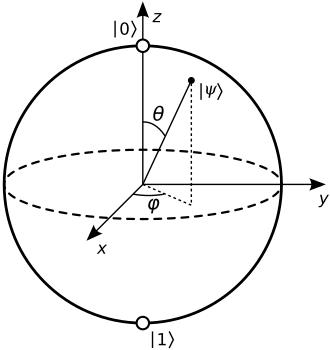
\includegraphics[width=0.3\textwidth]{img/Bloch/bloch_sphere.png}
        \caption{Esfera de Bloch. Obtenida de [Wikipedia]}\label{fig: bloch_sphere}
    \end{figure}

    Pudiendo representar todos los posibles estados de un qubit \( \ket{\psi} \) como un vector dentro de esta esfera. 
    Si nos fijamos en la expresión (\ref{eq: qubit_trigonometrico_esfera_bloch}) que acabamos de ver, vemos que hay un número complejo \( e^{i \varphi} \) de módulo uno, similar a una fase global. Sin embargo, esto no es una fase global, ya que para ello ha de multiplicar a todos los posibles estados del qubit, y vemos en este caso que solo aparece en el estado \( \ket{1} \), por lo que es una \textit{fase relativa}, y a diferencia de las fases globales que no cambian el significado físico del qubit, la fase relativa sí lo modifica. Esto es debido a que, aunque los coeficientes que acompañan a \( \ket{0} \) y \( \ket{1} \) sigan cumpliendo que su módulo al cuadrado sea uno, el vector representado en la esfera de Bloch es diferente, ya que puede variar el ángulo \( \varphi \).

    \vspace{5mm}

    Podemos pensar que aunque cambie la fase relativa no va a cambiar la probabilidad de obtener el estado \( \ket{0} \) o \( \ket{1} \) al medir el qubit. Esto se debe a que las mediciones se realizan normalmente sobre el eje \( Z \) y dicho vector estaría a la misma distancia de ambos polos de la esfera, manteniendo la probabilidad de obtener ambos estados \( \ket{0}, \ket{1} \) invariante, ya que la probabilidad de obtener un estado viene dada por el módulo al cuadrado de los coeficientes que los acompañan, como se puede apreciar en la expresión (\ref{eq: condicion_coeficientes_probabilidad_1}). Pero, ¿Y si cambiamos de base?
    
    \vspace{10mm}

    \subsection{Medición del Estado un Qubit}

    \vspace{5mm}

    Antes de hacer cambios de base, tenemos que tratar sobre las mediciones, las cuales ya hemos introducido en los párrafos anteriores y en esta pequeña sección vamos a profundizar sobre este tema. Como bien sabemos, un qubit puede estar en una superposición de \( \ket{0} \) y \( \ket{1} \) debido a las leyes de la mecánica cuántica, pero esto también establece que cuando vamos a leer el resultado de una operación, como al finalizar un algoritmo cuántico, este qubit colapsa a un único estado, de manera que obtenemos \( \ket{0} \) o bien \( \ket{1} \), cada uno con una cierta probabilidad, y esa probabilidad es el módulo al cuadrado de los coeficientes que acompañan a cada posible estado, como vimos en (\ref{eq: condicion_coeficientes_probabilidad_1}). Estos coeficientes se denominan amplitudes, y al tratarse de una probabilidad, la suma del módulo al cuadrado de las amplitudes ha de ser igual a uno. Vamos a ver esto con un ejemplo:

    \vspace{5mm}

    \begin{figure}[h!]
        \centering
        \begin{minipage}{0.3\textwidth}
            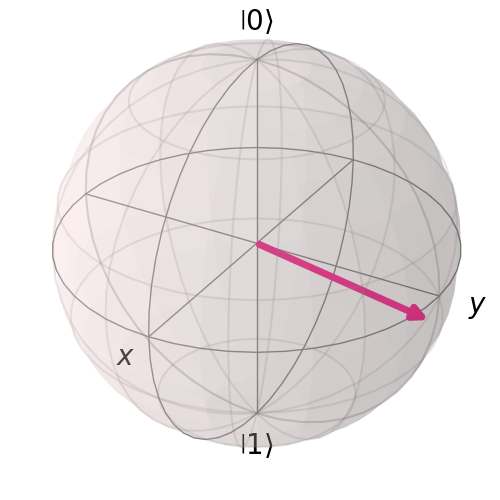
\includegraphics[width=\textwidth]{img/Bloch/bloch_measurement_example.png}  
        \end{minipage}
        \hfill
        \begin{minipage}{0.65\textwidth}
            Sea el siguiente qubit \( \ket{\psi} \):
            \begin{equation*}
                \ket{\psi} = \frac{1 + i \sqrt{3}}{3} \ket{0} + \frac{2 - i}{3} \ket{1}
            \end{equation*}
            La probabilidad de obtener el estado \( \ket{0} \) y el estado \( \ket{1} \) viene dada por 
            \begin{equation*}
                \left| \frac{1 + i \sqrt{3}}{3} \right| ^ {2} + \left| \frac{2 - i}{3} \right| ^ {2} = \left( \frac{1 + i \sqrt{3}}{3} \right) \left( \frac{1 - i \sqrt{3}}{3} \right) + \left( \frac{2 - i}{3} \right) \left( \frac{2 + i}{3} \right) =
            \end{equation*}
            \begin{equation*}
                \frac{4}{9} + \frac{5}{9} = 1
            \end{equation*}
        \end{minipage}
        \caption{Medición de un Qubit. Obtenida de [Qiskit]}\label{fig: bloch_ejemplo_medicion} 
    \end{figure}

    Siendo la probabilidad de colapsar en \( \ket{0} \) de \( \frac{4}{9} \) y de \( \frac{5}{9} \) en el estado \( \ket{1} \). Esto lo podemos ver gráficamente si representamos el vector correspondiente al estado \( \ket{\psi} \) en la esfera de Bloch, ya que si nos fijamos en (\ref{fig: bloch_ejemplo_medicion}) podemos ver que \( \ket{\psi} \) está un poco más cercano al estado \( \ket{1} \) de dicha esfera, y esto se corresponde con una probabilidad mayor de obtener dicho estado, como hemos podido apreciar en el ejemplo anterior.

    \vspace{5mm}

    Una vez definida correctamente la medición de un qubit, podemos hablar más profundamente sobre el concepto de \textit{colapso} de un qubit. Cuando medimos un qubit, este colapsa a un estado como hemos visto anteriormente, que puede ser \( \ket{0} \) o \( \ket{1} \) según el ejemplo propuesto, de manera que el estado del qubit se vuelve completamente fijo al estado que ha colapsado, por lo que el qubit deja de estar en superposición, y es forzado a tomar un bando, en este caso \( \ket{0} \) o \( \ket{1} \). Esto hace que el estado del qubit esté ya completamente definido, de manera que si volvemos a medir el estado de \( \ket{\psi} \), obtendremos el estado al que ha colapsado con una probabilidad de 1.

    \vspace{5mm}

    Tomando el ejemplo anterior, supongamos que \( \ket{\psi} \) colapsa a \( \ket{1} \). La probabilidad de que \( \ket{\psi} \) haya colapsado en \( \ket{1} \) es de \( \frac{5}{9} \) según la explicación anterior, sin embargo, si medimos el qubit una segunda vez, es decir, después de que haya colapsado, la probabilidad de obtener otra vez el mismo estado \( \ket{1} \) es 1, mientras que la probabilidad de obtener \( \ket{0} \) es 0. Esto es debido a que el qubit ya ha colapsado a un estado, por lo que podemos concluir que las mediciones de los qubits afectan a su estado físico, dejando de estar en superposición e influyendo el resultado de las mediciones posteriores. Es por esto que, generalmente, vamos a realizar las mediciones de los diferentes qubits al final de un algoritmo cuántico.

    \vspace{10mm}





    \subsection{Cambio de Base}

    \vspace{5mm}

    Generalmente, vamos a realizar las mediciones en el eje \( Z \), ya que los polos de este eje son los estados \( \ket{0} \) y \( \ket{1} \), que representan la información clásica de un bit, la cual sabemos que puede ser 0 o 1, por lo que efectivamente, toda la información clásica, o mejor dicho, todo algoritmo clásico se puede realizar mediante un algoritmo cuántico, simplemente haciendo una adaptación de puertas lógicas a puertas cuánticas como ya veremos más adelante. 

    \vspace{5mm}

    Ya sabemos la razón por la que vamos a medir en la mayoría de los casos sobre el eje \( Z \), pero como podemos apreciar en la esfera de Bloch, tenemos infinitos ejes sobre los que podríamos hacer la medición, así que la única condición para escoger dos puntos como vectores base de nuestro espacio de Hilbert \( \mathcal{H} \) sobre el que estudiaremos el estado de nuestro qubit \( \ket{\psi} \), es que estos puntos sean completamente opuestos. Vamos a tomar como ejemplo los estados en el eje \( X \) e \( Y \), cuyos polos son \( \ket{+}, \ket{-} \) y \( \ket{i}, \ket{-i} \), respectivamente

    \begin{figure}[H]
        \centering
        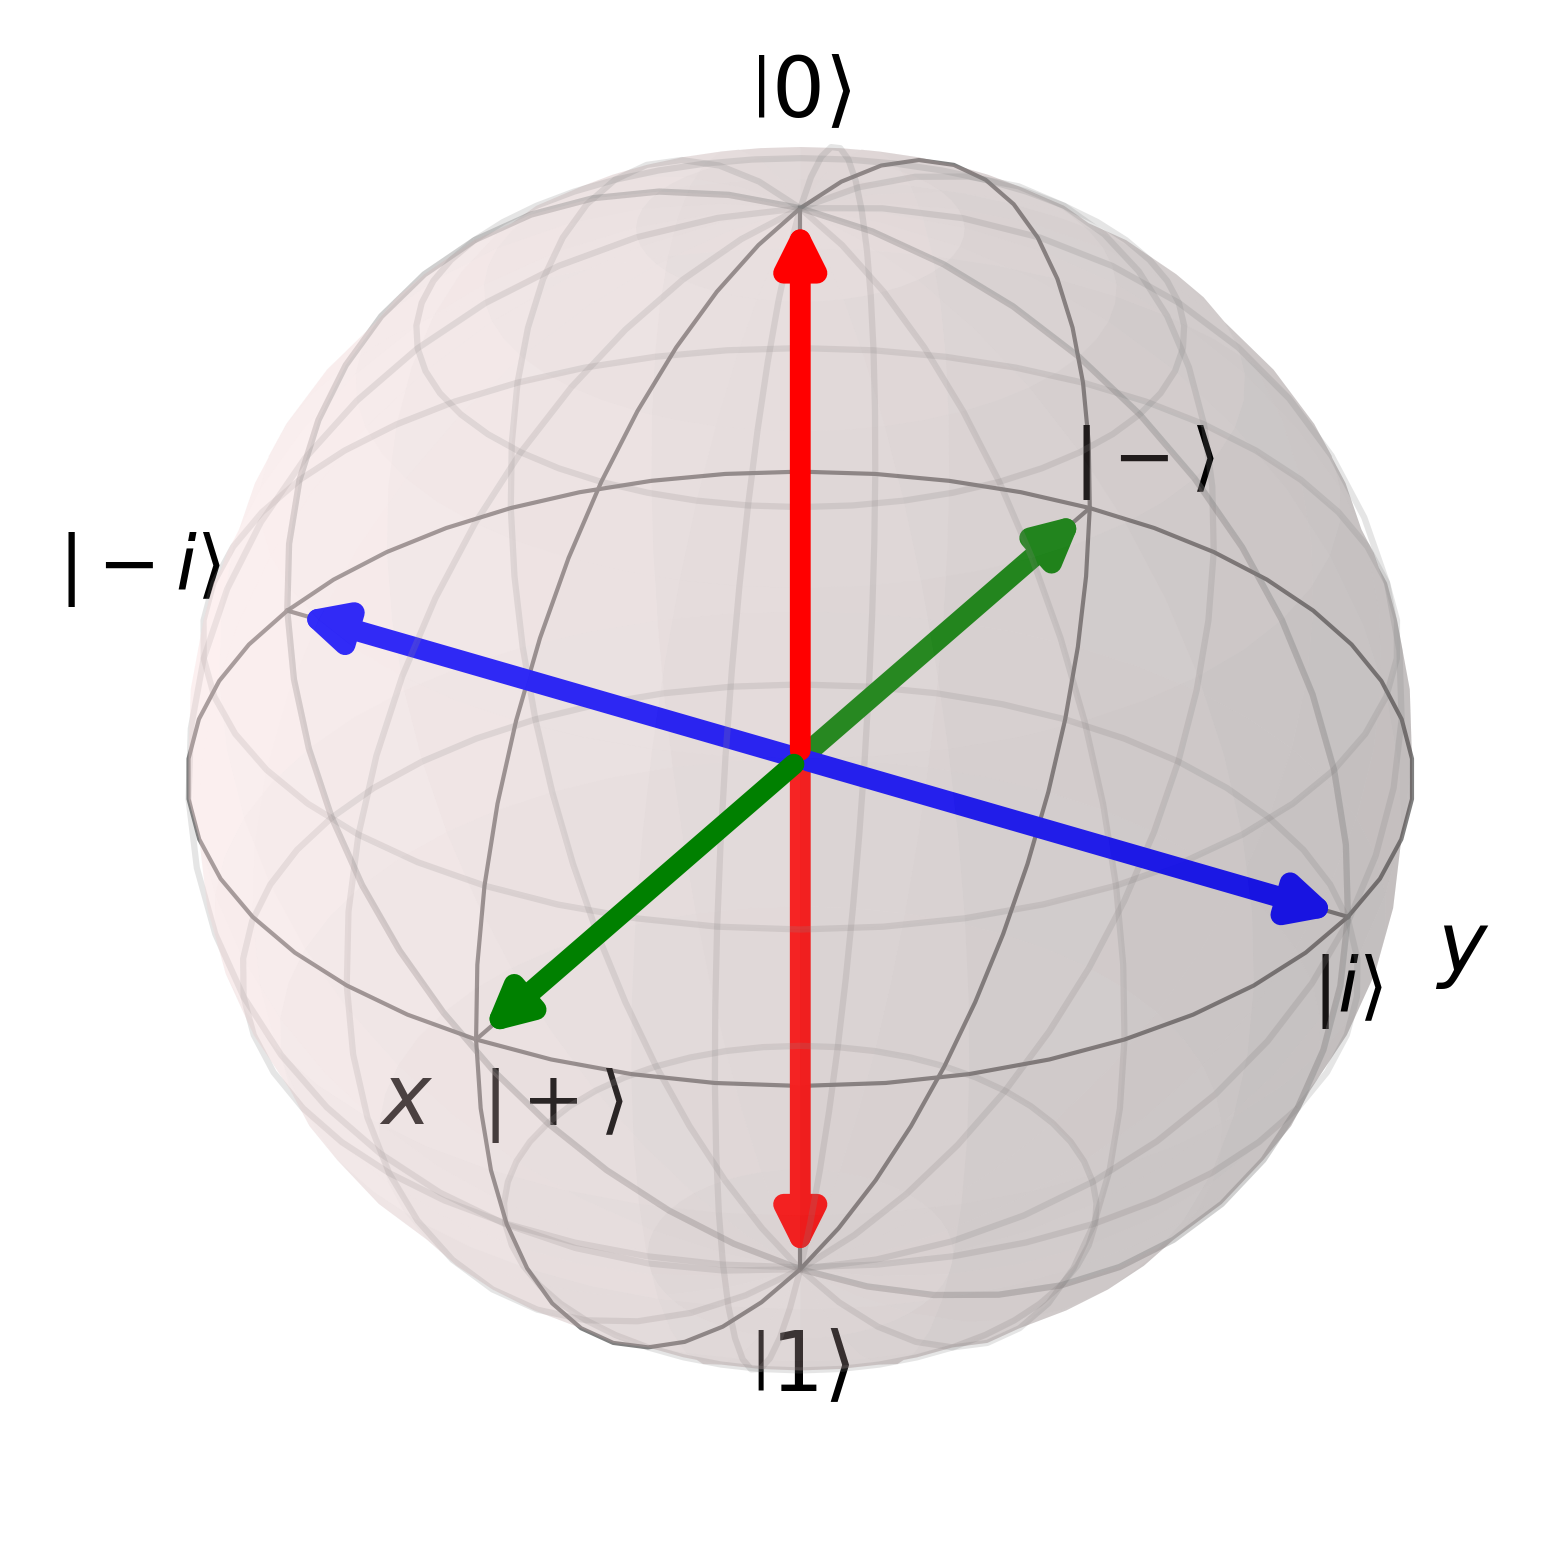
\includegraphics[width=0.3\textwidth]{img/Bloch/bloch_other_bases.png}
        \caption{Estados principales de la esfera de Bloch. Obtenida de [Qiskit]}\label{fig: bloch_other_bases}
    \end{figure}

    Estos estados se pueden expresar en base a \( \ket{0} \) y \( \ket{1} \):

    \begin{align}
        \label{eq: estados_eje_x_y}
        \ket{+} &= \frac{1}{\sqrt{2}} \left( \ket{0} + \ket{1} \right) \\[10pt]
        \ket{-} &= \frac{1}{\sqrt{2}} \left( \ket{0} - \ket{1} \right) \\[10pt]
        \ket{i} &= \frac{1}{\sqrt{2}} \left( \ket{0} + i\ket{1} \right) \\[10pt]
        \ket{-i} &= \frac{1}{\sqrt{2}} \left( \ket{0} - i\ket{1} \right)
    \end{align}

    \vspace{2.5mm}

    Y su representación la podemos ver reflejada en (\ref{fig: bloch_other_bases}). Estos estados sabemos que están en superposición ya que no se encuentran en \( \ket{0} \) o \( \ket{1} \), de hecho, están justamente en el punto medio entre \( \ket{0} \) y \( \ket{1} \), por lo que la probabilidad de obtener \( \ket{0} \) o \( \ket{1} \) es exactamente la misma (\( \frac{1}{2} \)) si nuestro qubit \( \ket{\psi} \) se encuentra en uno de los estados en (\ref{eq: estados_eje_x_y}). No obstante, para poder realizar el cambio de base, necesitamos expresar los estados \( \ket{0} \) y \( \ket{1} \) en función de la base a la que queramos aplicar el cambio. Comencemos por \( \ket{+} \) y \( \ket{-} \):

    \begin{equation}
        \ket{+} + \ket{-} = \frac{1}{\sqrt{2}} \left( \ket{0} + \ket{1} \right) + \frac{1}{\sqrt{2}} \left( \ket{0} - \ket{1} \right) = \frac{2}{\sqrt{2}} \ket{0} = \sqrt{2} \ket{0} \ \implies \ \boxed{\ket{0} = \frac{1}{\sqrt{2}} \left( \ket{+} + \ket{-} \right)} 
        \label{eq: estado_0_en_funcion_mas_menos}
    \end{equation}
    \begin{equation}
        \ket{+} - \ket{-} = \frac{1}{\sqrt{2}} \left( \ket{0} + \ket{1} \right) - \frac{1}{\sqrt{2}} \left( \ket{0} - \ket{1} \right) = \frac{2}{\sqrt{2}} \ket{1} = \sqrt{2} \ket{1} \ \implies \ \boxed{\ket{1} = \frac{1}{\sqrt{2}} \left( \ket{+} - \ket{-} \right)}
        \label{eq: estado_1_en_funcion_mas_menos}
    \end{equation}

    \vspace{5mm}

    Y esto está muy relacionado con la \textit{puerta de Hadamard}, la cual es una de las puertas cuánticas de un qubit más importantes, como veremos en la siguiente sección. Volviendo a retomar el ejemplo (\ref{fig: bloch_ejemplo_medicion}), vamos a aplicar el cambio a la base \( B_{H} = \left\{ \ket{+}, \ket{-} \right\}\) y ver como afecta esto al estado de nuestro qubit \( \ket{\psi} \). Aplicando dicho cambio, nos queda lo siguiente

    \begin{figure}[h!]
        \centering
        \begin{minipage}{0.65\textwidth}
            \begin{align*}
                &\ket{\psi} = \frac{1 + i \sqrt{3}}{3} \ket{0} + \frac{2 - i}{3} \ket{1} = \frac{1 + i \sqrt{3}}{3 \sqrt{2}} \left( \ket{+} + \ket{-} \right) + \frac{2 - i}{3 \sqrt{2}} \left( \ket{+} - \ket{-} \right) = \\[10pt]
                &= \frac{3 + \left( \sqrt{3} - 1 \right) i}{3 \sqrt{2}} \ket{+} - \frac{1 - \left( \sqrt{3} + 1 \right) i}{3 \sqrt{2}} \ket{-}
            \end{align*}
            Y la probabilidad de obtener \( \ket{+} \) y \( \ket{-} \) es 
            \begin{align*}
                \ket{+} \ &\longrightarrow \ \left| \ \frac{3 + \left( \sqrt{3} - 1 \right) i}{3 \sqrt{2}} \ \right| ^ {2} = \frac{9 + \left( \sqrt{3} - 1\right) ^ {2}}{18} \approx 0.53 \\[10pt]
                \ket{-} \ &\longrightarrow \ \left| \ \frac{1 - \left( \sqrt{3} + 1 \right) i}{3 \sqrt{2}} \ \right| ^ {2} = \frac{1 + \left( \sqrt{3} + 1\right) ^ {2}}{18} \approx 0.47
            \end{align*}
        \end{minipage}
        \hfill
        \begin{minipage}{0.3\textwidth}
            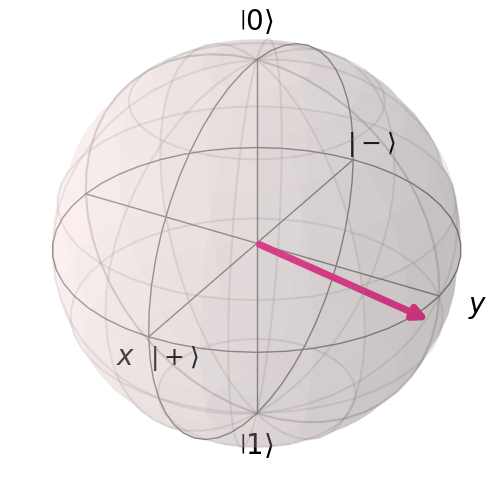
\includegraphics[width=\textwidth]{img/Bloch/bloch_change_basis_example.png}  
        \end{minipage}
        \caption{Cambio de base. Obtenida de [Qiskit]}\label{fig: bloch_ejemplo_medicion_2} 
    \end{figure}

    \vspace{10mm}

    Podemos ver que esto tiene sentido, ya que el vector que representa el estado de \( \ket{\psi} \) se encuentra ligeramente más próximo al estado \( \ket{+} \) que a \( \ket{-} \), por lo que es lógico obtener una probabilidad en \( \ket{+} \) ligeramente mayor que en \( \ket{-} \), aunque esto no quiere decir que vaya a colapsar siempre a \( \ket{+} \), significa que si midiéramos varios qubits en el mismo estado que \( \ket{\psi} \), por estadísitica, obtendríamos normalmente mayor número de colapsos en \( \ket{+} \), aunque no siempre va a colapsar en \( \ket{+} \) por tener una probabilidad mayor.

    \vspace{5mm}

    De la misma manera que en (\ref{eq: estado_0_en_funcion_mas_menos}) y (\ref{eq: estado_1_en_funcion_mas_menos}), podemos expresar \( \ket{0} \) y \( \ket{1} \) en función de \( \ket{i} \) y \( \ket{-i} \), obteniendo que

    \begin{equation}
        \ket{0} = \frac{1}{\sqrt{2}} \left( \ket{i} + \ket{-i} \right), \quad \ket{1} = \frac{-i}{\sqrt{2}} \left( \ket{i} - \ket{-i} \right) 
        \label{eq: estado_0_y_1_en_funcion_i_menosi}
    \end{equation}

    \vspace{5mm}

    En este caso la diferencia entre ambas probabilidades va a ser mucho mayor, ya que \( \ket{\psi} \) está muy próximo a \( \ket{i} \) en la esfera de Bloch, por lo que la probabilidad de obtener \( \ket{i} \) será muy cercana a uno, y en caso contrario, la probabilidad de obtener \( \ket{-i} \) será prácticamente nula.

    \begin{figure}[h!]
        \centering
        \begin{minipage}{0.3\textwidth}
            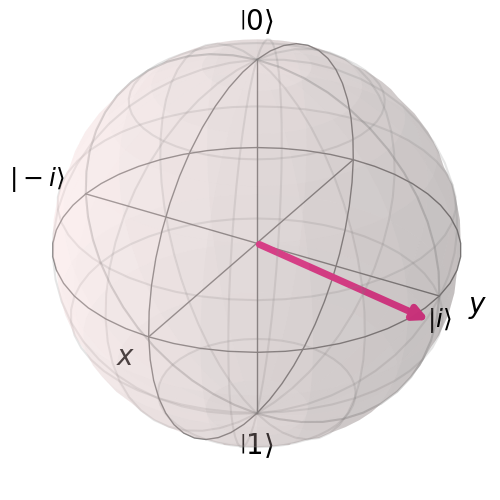
\includegraphics[width=\textwidth]{img/Bloch/bloch_change_basis_example_2.png}  
        \end{minipage}
        \hfill
        \begin{minipage}{0.65\textwidth}
            \begin{align*}
                &\ket{\psi} = \frac{1 + i \sqrt{3}}{3} \ket{0} + \frac{2 - i}{3} \ket{1} = \frac{1 + \sqrt{3}i}{3 \sqrt{2}} \left( \ket{i} + \ket{-i} \right) - \frac{1 + 2i}{3 \sqrt{2}} \left( \ket{i} - \ket{-i} \right) = \\[10pt]
                &=  \frac{\left( \sqrt{3} - 2 \right)i}{3 \sqrt{2}} \ket{i} + \frac{2 + \left( \sqrt{3} + 2 \right) i}{3 \sqrt{2}} \ket{-i}
            \end{align*}
            Y la probabilidad de obtener \( \ket{i} \) y \( \ket{-i} \) es
            \begin{align*}
                \ket{i} \ &\longrightarrow \ \left| \ \frac{\left( \sqrt{3} - 2 \right) i}{3 \sqrt{2}} \ \right| ^ {2} = \frac{\left( \sqrt{3} - 2 \right) ^ {2}}{18} \approx 0.004 \\[10pt]
                \ket{-i} \ &\longrightarrow \ \left| \ \frac{2 + \left( \sqrt{3} + 2 \right) i}{3 \sqrt{2}} \ \right| ^ {2} = \frac{4 + \left( \sqrt{3} + 2 \right) ^ {2}}{18} \approx 0.996
            \end{align*}
        \end{minipage}
        \caption{Cambio de base. Obtenida de [Qiskit]}\label{fig: bloch_ejemplo_medicion_3} 
    \end{figure}

    Perfecto, vemos que el resultado es el esperado. Ahora, estamos en condiciones de explicar la fase relativa correctamente. Al final de (\ref{sec: el_qubit}), explicamos que una fase global no modifica el estado físico de un qubit, pero dejamos un poco abierta la fase relativa. Vamos a volver a trabajar sobre el estado de un qubit puro definido en (\ref{eq: qubit_trigonometrico_esfera_bloch}), definiendo las probabilidades de medir \( \ket{\psi} \) sobre el eje \( Z \) y posteriormente sobre el eje \( X \), y nos vamos a dar cuenta que las probabilidades no coinciden, concluyendo en que una fase relativa sí que modifica el estado físico de un qubit, a diferencia de una fase global. Comencemos por la probabilidad de obtener \( \ket{0} \) y \( \ket{1} \)
    \begin{equation*}
        &\ket{\psi} = \cos \left( \frac{\theta}{2} \right) \ket{0} + e^{i \varphi} \sin \left( \frac{\theta}{2} \right) \ket{1}
    \end{equation*}
    \begin{align*}
        &\ket{0} \ \longrightarrow \ \left| \cos \left( \frac{\theta}{2} \right) \right| ^ {2} = \cos^{2} \left( \frac{\theta}{2} \right) \\[10pt]
        &\ket{1} \ \longrightarrow \ \left| e^{i \varphi} \sin \left( \frac{\theta}{2} \right) \right| ^ {2} = \left( \cos \left( \frac{\theta}{2} \right) + i \sin \left( \frac{\theta}{2} \right) \right)\right| \left( \cos \left( \frac{\theta}{2} \right) - i \sin \left( \frac{\theta}{2} \right) \right)\right| \sin^{2} \left( \frac{\theta}{2} \right) = \sin^{2} \left( \frac{\theta}{2} \right)
    \end{align*}

    \vspace{2.5mm}

    Ahora, haciendo el cambio de base a \( \left\{ \ket{0}, \ket{1} \right\} \)
    \begin{equation*}
        \ket{\psi} = \frac{1}{\sqrt{2}} \cos \left( \frac{\theta}{2} \right) \left( \ket{+} + \ket{-} \right) + \frac{1}{\sqrt{2}} + \frac{1}{\sqrt{2}} e^{i \varphi} \sin \left( \frac{\theta}{2} \right) \left( \ket{+} - \ket{-} \right) = 
    \end{equation*}
    \begin{equation*}
        = \left[ \frac{1}{\sqrt{2}} \cos \left( \frac{\theta}{2} \right) + \frac{1}{\sqrt{2}} e^{i \varphi} \sin \left( \frac{\theta}{2} \right) \right] \ket{+} + \left[ \frac{1}{\sqrt{2}} \cos \left( \frac{\theta}{2} \right) - \frac{1}{\sqrt{2}} e^{i \varphi} \sin \left( \frac{\theta}{2} \right) \right] \ket{-} 
    \end{equation*}

    \vspace{2.5mm}

    Vemos que las probabilidades no son las mismas que con la base anterior:
    \begin{align*}
        \ket{+} \ &\longrightarrow \ \left| \frac{1}{\sqrt{2}} \cos \left( \frac{\theta}{2} \right) + \frac{1}{\sqrt{2}} e^{i \varphi} \sin \left( \frac{\theta}{2} \right) \right| ^ {2} = \frac{1}{2} \left[ \cos \left( \frac{\theta}{2} \right) + \sin \left( \frac{\theta}{2} \right)\right] ^ {2} \\[10pt]
        \ket{-} \ &\longrightarrow \ \left| \frac{1}{\sqrt{2}} \cos \left( \frac{\theta}{2} \right) - \frac{1}{\sqrt{2}} e^{i \varphi} \sin \left( \frac{\theta}{2} \right) \right| ^ {2} = \frac{1}{2} \left[ \cos \left( \frac{\theta}{2} \right) - \sin \left( \frac{\theta}{2} \right)\right] ^ {2}
    \end{align*}

    \vspace{5mm}

    Por lo que hemos comprobado que una fase relativa no altera el estado de un qubit \( \ket{\psi} \) en el eje \( Z \), sino que lo hace en el plano azimutal, de manera que al medir el estado de \( \ket{\psi} \) en otra base como \( \{ \ket{+}, \ket{-} \} \), la probabilidad de colapso cambia. Esto no sucede cuando aplicamos una fase global.

    \vspace{10mm}


    


    \subsection{Puertas Cuánticas}\label{sec: puertas_cuanticas}

    \vspace{5mm}

    Habiendo introducido la unidad de información cuántica y sus respectivas mediciones sobre los ejes \( X \), \( Y \) y \( Z \), estamos ya en condiciones de estudiar las puertas cuánticas. Así como las puertas lógicas en computación clásica son capaces de modificar la información que reside en los distintos bits, las puertas cuánticas actúan sobre el estado físico de los respectivos qubits, siguiendo las leyes de la mecánica cuántica como hemos visto hasta ahora, de manera que se consigue modificar el estado de un qubit \( \ket{\psi} \) como resultado de una operación, por ejemplo, desencriptar las claves públicas y privadas de un cifrado de información, como veremos más adelante.
    
    \vspace{5mm}

    Estas puertas cuánticas, las podemos representar como matrices, aprovechando todo el álgebra lineal que llevamos impartido hasta ahora. Realmente, pudimos haber representado el estado de un qubit \( \ket{\psi} \) en la sección anterior como un vector columna, aprovechando la representación matricial de \( \ket{0} \) y \( \ket{1} \) que sigue como

    \begin{equation}
        \ket{0} = \begin{pmatrix}
            1 \\
            0
        \end{pmatrix}
        , \quad \ket{1} = \begin{pmatrix}
            0 \\
            1
        \end{pmatrix}
    \end{equation}

    \vspace{2.5mm}

    Si tomamos el estado de un qubit puro que definimos en (\ref{eq: combinacion_lineal_estados_1_qubit}), vemos que podemos definir el estado de un qubit cualquiera \( \ket{\psi} \) como un vector columna de dimensión \( 2^{N} \), siendo \( N \) el número de qubits de nuestro computador cuántico, por lo que para un sistema cuántico de un único qubit tenemos el siguiente vector:

    \begin{equation}
        \ket{\psi} = \alpha \ket{0} + \beta \ket{1} = \alpha \begin{pmatrix}
        1 \\
        0
        \end{pmatrix} + \beta \begin{pmatrix}
        0 \\
        1
        \end{pmatrix} = \begin{pmatrix}
        \alpha \\
        \beta
        \end{pmatrix}
        \label{eq: vector_sistema_un_qubit}
    \end{equation}

    \vspace{2.5mm}

    De esta manera, podemos expresar el estado de cualquier qubit como un vector columna de dimensión 2, y ya veremos la generalización de esta representación vectorial para \( N \) qubits en la siguiente sección (\ref{sec: multiples_qubits}). Por otra parte, vamos ya a afrontar las puertas cuánticas, las cuales no son más que operadores sobre un espacio de Hilbert \( \mathcal{H} \) que transforman el estado de un qubit en otro estado diferente, como vimos en (\ref{eq: operador_espacio_hilbert}):

    \begin{equation*}
        \hat{A} \ket{\psi} \overset{\hat{A}}{\longrightarrow} \ket{\psi '}, \qquad \ket{\psi}, \ket{\psi '} \in \mathcal{H}
    \end{equation*}

    \vspace{2.5mm}

    Para estos operadores ser bautizados como puertas cuánticas, han de satisfacer unas ciertas condiciones. La primera es la condición de linealidad, la cual establece que

    \begin{equation}
        U \left( \alpha \ket{0} + \beta \ket{1} \right) = \alpha U \ket{0} + \beta U \ket{1}
        \label{eq: linealidad_puertas_cuanticas}
    \end{equation}

    \vspace{2.5mm}

    La segunda es que la probabilidad total de los estados a obtener en una medición ha de seguir manteniéndose uno, como vimos en el capítulo anterior en (\ref{eq: condicion_coeficientes_probabilidad_1})

    \begin{equation*}
        | \alpha | ^ {2} + | \beta | ^ {2} = 1
    \end{equation*}

    \vspace{2.5mm}

    Para ver qué tipo de matrices satisfacen esta propiedad, vamos a apoyarnos en el conjugado hermítico. Sea la siguiente puerta cuántica \( U \):

    \begin{equation*}
        U = \begin{pmatrix}
            a & c \\
            b & d
        \end{pmatrix}
    \end{equation*}

    \vspace{2.5mm}

    Si la aplicamos sobre un qubit \( \ket{\psi} \), nos queda como resultado un qubit diferente, el cual denotaremos como \( \ket{U \psi} \)

    \begin{equation}
        U \ket{\psi} = \begin{pmatrix}
            a & c \\
            b & d
        \end{pmatrix} \begin{pmatrix}
            \alpha \\
            \beta
        \end{pmatrix} = \begin{pmatrix}
            a \alpha + c \beta \\
            b \alpha + d \beta
        \end{pmatrix} = \ket{U \psi}
    \label{eq: puerta_cuantica_vector_aplicado}
    \end{equation}

    \vspace{2.5mm}

    Si ahora consideramos el conjugado hermítico de \( \ket{U \psi} \), el cual definimos en la introducción de los espacios de Hilbert \( \mathcal{H} \) en (\ref{eq: conjugado_hermitico}), tenemos que

    \begin{equation}
        \bra{U \psi} = \begin{pmatrix}
            a^{*} \alpha^{*} + c^{*} \beta^{*} & b^{*} \alpha^{*} + d^{*} \beta^{*} 
        \end{pmatrix} = \begin{pmatrix}
            \alpha^{*} & \beta^{*}
        \end{pmatrix} \begin{pmatrix}
            a^{*} & d^{*} \\
            c^{*} & d^{*}
        \end{pmatrix} = \begin{pmatrix}
            \alpha^{*} & \beta^{*}
        \end{pmatrix} \begin{pmatrix}
            a & c \\
            b & d
        \end{pmatrix} ^ {\dagger} = \bra{\psi} U^{\dagger}
    \label{eq: puerta_cuantica_conjugado_hermitico}
    \end{equation}

    \vspace{2.5mm}

    Entonces, apoyándonos en las propiedades que acabamos de ver (\ref{eq: puerta_cuantica_vector_aplicado}) y (\ref{eq: puerta_cuantica_conjugado_hermitico}), obtenemos finalmente la segunda condición que estamos buscando. Esto lo hacemos viendo que el producto escalar de \( \ket{U \psi} \) sobre sí mismo, es decir, la proyección de \( \ket{U \psi} \) sobre sí mismo, es igual a 1:
    \begin{align}
        \braket{U \psi \ | \ U \psi} &= 1 \nonumber \\[10pt]
        \braket{\psi | U^{\dagger} U | \psi} &= \braket{\psi \ | \ \psi} \nonumber \\[10pt]
        U^{\dagger} U &= I
        \label{eq: puertas_cuanticas_unitarias}
    \end{align}

    Y las matrices que satisfacen esta última propiedad (\ref{eq: puertas_cuanticas_unitarias}) se conocen como \textit{unitarias}, y podemos afirmar algo muy importante, y es que toda matriz unitaria es una puerta cuántica, y toda puerta cuántica es una matriz unitaria. Además, como hemos podido ver en (\ref{eq: puertas_cuanticas_unitarias}), \( U^{\dagger} \) es la matriz inversa de \( U \), ya que el producto de estas dos matrices da como resultado la matriz identidad \( I \), por lo que toda puerta cuántica \( U \) es reversible, y su matriz inversa es su conjugado hermítico \( U^{\dagger} \), de manera que si aplicamos una puerta cuántica \( U \) sobre un qubit \( \ket{\psi} \), podemos volver al estado original de \( \ket{\psi} \) aplicando \( U^{\dagger} \)

    \begin{equation*}
        U^{\dagger} U \ket{\psi} = U U^{\dagger} \ket{\psi} = I \ket{\psi} = \ket{\psi}
    \end{equation*}

    \vspace{2.5mm}

    Esta última condición tiene mucho que ver con que las puertas cuánticas tienen que ser reversibles, es decir, siempre hemos de saber de que estado proviene el resultado. Para ver esto mejor, vamos a apoyarnos en las puertas lógicas clásicas, en este caso la puerta \textit{NOT}, cuya tabla de verdad es

    \begin{table}[h!]
        \centering
        \begin{tabular}{|c|c|}
            \hline
            A & B \\
            \hline
            0 & 1 \\
            1 & 0 \\
            \hline
        \end{tabular}
        \caption{Puerta lógica NOT.}
        \label{table: puerta_clasica_not}
    \end{table}

    Si obtenemos el resultado \( B = 1 \), sabemos que el bit antes de aplicar la puerta era \( 0 \), y si obtenemos \( B = 0 \), no queda otra opción que el bit fuese \( 1 \), esto lo podemos representar como una matriz:
    
    \begin{equation*}
        \begin{array}{l}
            \ket{0} \rightarrow 1 \\
            \ket{1} \rightarrow 0  
        \end{array}
        \left\}
        \quad
        \text{NOT} =
        \begin{pmatrix}
            0 & 1 \\
            1 & 0
        \end{pmatrix}
    \end{equation*}

    \vspace{2.5mm}

    Y esta matriz vemos que es unitaria, ya que su matriz conjugada transpuesta por ella misma es la identidad \( I \)

    \begin{equation*}
        \begin{pmatrix}
            0 & 1 \\
            1 & 0
        \end{pmatrix} \begin{pmatrix}
            0 & 1 \\
            1 & 0
        \end{pmatrix} ^ {\dagger} = \begin{pmatrix}
            0 & 1 \\
            1 & 0
        \end{pmatrix} \begin{pmatrix}
            0 & 1 \\
            1 & 0
        \end{pmatrix} = I
    \end{equation*}

    \vspace{2.5mm}

    Por lo que la puerta clásica \textit{NOT} es una puerta cuántica perfectamente válida, la cual explicaremos en el siguiente apartado. Para ver el caso contrario, vamos a suponer la puerta clásica cuyo resultado es siempre 1:
    
    \begin{table}[h!]
        \centering
        \begin{tabular}{|c|c|}
            \hline
            A & B \\
            \hline
            0 & 1 \\
            1 & 1 \\
            \hline
        \end{tabular}
        \caption{Puerta lógica clásica constante a 1.}
        \label{table: puerta_clasica_todo_1}
    \end{table}

    Y  podemos verificar que la matriz que representa a esta puerta no es unitaria
        
    \begin{equation*}
        \begin{pmatrix}
            0 & 0 \\
            1 & 1
        \end{pmatrix} \begin{pmatrix}
            0 & 0 \\
            1 & 1
        \end{pmatrix} ^ {\dagger} = \begin{pmatrix}
            0 & 0 \\
            1 & 1
        \end{pmatrix} \begin{pmatrix}
            0 & 1 \\
            0 & 1
        \end{pmatrix} =  \begin{pmatrix}
            0 & 0 \\
            0 & 1
        \end{pmatrix} \neq I
    \end{equation*}

    \vspace{2.5mm}

    Por lo que la puerta (\ref{table: puerta_clasica_todo_1}) no es una puerta cuántica. Este pequeño nos ayuda a entender mejor que toda puerta lógica clásica reversible tiene su contrapartida en computación cuántica, y el significado físico de estas puertas cuánticas lo vamos a ver a continuación con las puertas cuánticas de 1 qubit más importantes.

    \vspace{10mm}





    \subsection{Puertas Cuánticas de 1 Qubit}\label{subsection: puertas_cuanticas_de_1_qubit}

    \vspace{5mm}

    Una vez explicadas las condiciones que ha de cumplir una puerta cuántica, que son la condición de linealidad (\ref{eq: linealidad_puertas_cuanticas}) y que ha de ser unitaria, como vimos en (\ref{eq: puertas_cuanticas_unitarias}), vamos a tomar como ejemplo la puerta \textit{NOT} clásica, que tiene su contrapartida cuántica, la cual se suele denotar como \textit{X}, ya que cumple con los requisitos propuestos anteriormente, de manera que un qubit en el estado \( \ket{0} \) pasa a \( \ket{1} \) y viceversa:

    \begin{equation*}
        & X \ket{\psi} = \alpha X \ket{0} + \beta  X \ket{1} = \alpha \begin{pmatrix}
            0 & 1 \\
            1 & 0 
        \end{pmatrix} \begin{pmatrix}
            1 \\
            0
        \end{pmatrix} + \beta \begin{pmatrix}
            0 & 1 \\
            1 & 0 
        \end{pmatrix} \begin{pmatrix}
            0 \\ 
            1
        \end{pmatrix} = \alpha \begin{pmatrix}
            0 \\
            1
        \end{pmatrix} + \beta \begin{pmatrix}
            1 \\
            0
        \end{pmatrix} = \beta \ket{0} + \alpha \ket{1} 
    \end{equation*}

    \vspace{2.5mm}

    De esta manera, si aplicamos la puerta \textit{X} sobre un qubit \( \ket{\psi} \) que se encuentra en el estado \( \ket{0} \), esta puerta rota el estado del qubit \( \ket{\psi} \) al estado \( \ket{1} \)

    \vspace{5mm}

    \begin{minipage}{0.1\textwidth}
        \hfill
    \end{minipage}
    \begin{minipage}{0.3\textwidth}
        \centering
        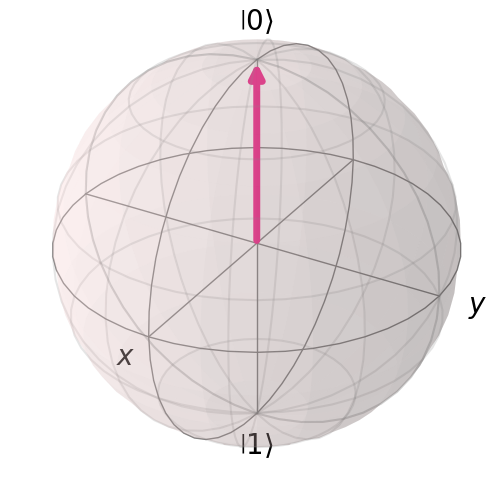
\includegraphics[width=\textwidth]{img/Bloch/bloch_state_0.png}
        \caption{Figura 9: Estado $|0\rangle$ en la esfera de Bloch. Obtenida de [Qiskit]}
    \end{minipage}
    \hfill
    \scalebox{2}{\(\overset{X}{\longrightarrow}\)}
    \hfill
    \begin{minipage}{0.3\textwidth}
        \centering
        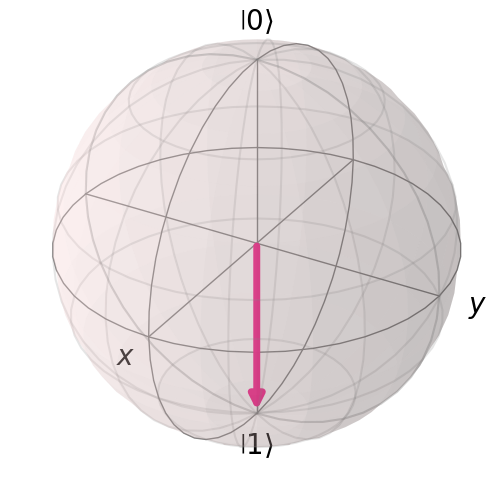
\includegraphics[width=\textwidth]{img/Bloch/bloch_state_1.png}
        \caption{Figura 10: Estado $|1\rangle$ en la esfera de Bloch. Obtenida de [Qiskit]}
    \end{minipage}
    \begin{minipage}{0.1\textwidth}
        \hfill
    \end{minipage}

    \vspace{5mm}

    Y esto ocurre también para el caso contrario. Esta puerta \textit{X} es una de las \textit{puertas de Pauli}, en concreto sobre el eje X, como su propio nombre indica, y también podemos definir las puertas de Pauli para el eje \textit{Y} y \textit{Z} de la esfera de Bloch, de la siguiente manera

    \begin{equation}
        X = \begin{pmatrix}
            0 & 1 \\
            1 & 0 
        \end{pmatrix}, \qquad Y = \begin{pmatrix}
            0 & -i \\
            i & 0
        \end{pmatrix}, \qquad Z = \begin{pmatrix}
            1 & 0 \\
            0 & -1
        \end{pmatrix}
        \label{eq: puertas_pauli}
    \end{equation}

    \vspace{2.5mm}

    Estas \textit{puertas de Pauli}, y de hecho, toda puerta cuántica de un único qubit representa una rotación de \( \ket{\psi} \) en la esfera de Bloch, esto es lógico ya que, como vimos anteriormente, toda puerta cuántica es un operador lineal que actúa sobre un qubit \( \ket{\psi} \), de manera que cambiamos el estado de dicho qubit \( \ket{\psi} \) a otro estado diferente \( \ket{\psi'} \), cuya norma sigue siendo la unidad, por lo que podemos visualizar muy bien la rotación en la esfera de Bloch. Así, las puertas de Pauli que acabamos de ver en (\ref{eq: puertas_pauli}) son rotaciones de \( \pi \) radianes sobre uno de los ejes de la esfera de Bloch. Veamos como actúa \textit{Y} sobre \( \ket{0} \):

    \begin{equation*}
        Y \ket{\psi} = \begin{pmatrix}
            0 & -i \\
            i & 0
        \end{pmatrix} \begin{pmatrix}
            1 \\
            0
        \end{pmatrix} = \begin{pmatrix}
            0 \\
            i
        \end{pmatrix} = i \begin{pmatrix}
            0 \\
            1
        \end{pmatrix} = i \ket{1}
    \end{equation*}

    \vspace{2.5mm}

    Y esto es el estado \( \ket{1} \) multiplicado por una fase global, en este caso \( i \), por lo que podemos eliminar la fase global, ya que esta no altera el significado físico de \( \ket{1} \), dándose por realizada la rotación esperada sobre el eje \textit{Y}

    \vspace{5mm}

    \begin{minipage}{0.1\textwidth}
        \hfill
    \end{minipage}
    \begin{minipage}{0.3\textwidth}
        \centering
        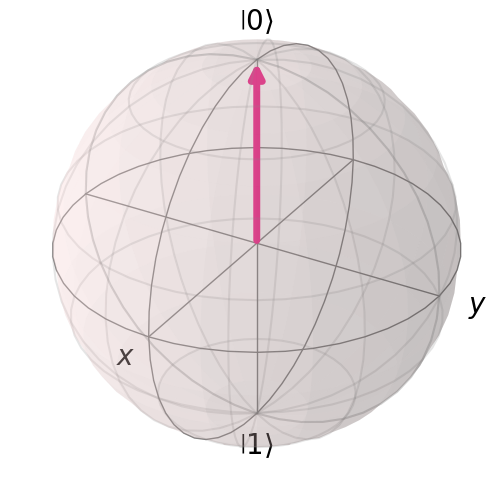
\includegraphics[width=\textwidth]{img/Bloch/bloch_state_0.png}
        \caption{Figura 11: Estado $|0\rangle$ en la esfera de Bloch. Obtenida de [Qiskit]}
    \end{minipage}
    \hfill
    \scalebox{2}{\(\overset{Y}{\longrightarrow}\)}
    \hfill
    \begin{minipage}{0.3\textwidth}
        \centering
        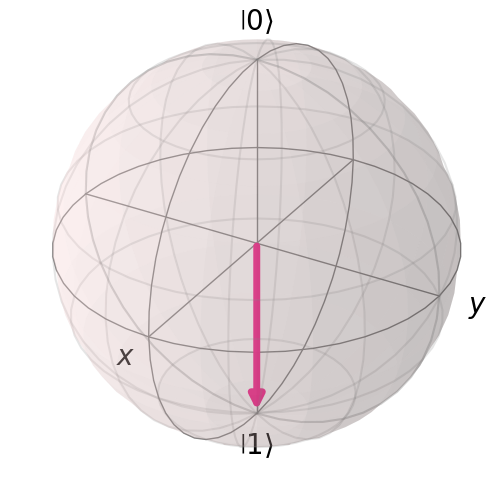
\includegraphics[width=\textwidth]{img/Bloch/bloch_state_1.png}
        \caption{Figura 12: Estado $|1\rangle$ en la esfera de Bloch. Obtenida de [Qiskit]}
    \end{minipage}
    \begin{minipage}{0.1\textwidth}
        \hfill
    \end{minipage}

    \vspace{5mm}

    Vamos a tomar como último ejemplo la puerta \textit{Z}, de manera que si la aplicamos sobre un qubit en \( \ket{0} \)
    el estado del qubit no cambia, ya que estamos aplicando una rotación sobre el eje \textit{Z}:

    \begin{equation*}
        Z \ket{0} = \begin{pmatrix}
            1 & 0 \\
            0 & -1
        \end{pmatrix} \begin{pmatrix}
            1 \\
            0
        \end{pmatrix} = \begin{pmatrix}
            1 \\
            0
        \end{pmatrix} = \ket{0}
    \end{equation*}

    \vspace{2.5mm}

    Como habíamos presupuesto anteriormente. A partir de estas puertas podemos crear todas las demás puertas cuánticas de 1 qubit. Vamos definir una puerta muy importante, la cual es una rotación sobre el eje \( X + Z \), que la podemos obtener únicamente sumando las puertas de Pauli \textit{X} y \textit{Z}

    \begin{equation*}
        X + Z = \begin{pmatrix}
            0 & 1 \\
            1 & 0 
        \end{pmatrix} + \begin{pmatrix}
            1 & 0 \\
            0 & -1
        \end{pmatrix} = \begin{pmatrix}
            1 & 1 \\
            1 & -1
        \end{pmatrix}
    \end{equation*}

    \vspace{2.5mm}

    Pero si nos fijamos esta matriz no es unitaria, ya que

    \begin{equation*}
        \begin{pmatrix}
            1 & 1 \\
            1 & -1
        \end{pmatrix} \begin{pmatrix}
            1 & 1 \\
            1 & -1
        \end{pmatrix} ^ {\dagger} = \begin{pmatrix}
            1 & 1 \\
            1 & -1
        \end{pmatrix} \begin{pmatrix}
            1 & 1 \\
            1 & -1
        \end{pmatrix} = \begin{pmatrix}
            2 & 0 \\
            0 & 2
        \end{pmatrix} = 2 \ I \neq I
    \end{equation*}

    \vspace{2.5mm} 

    Para que sea unitaria hemos de multiplicar la matriz por \( \frac{1}{\sqrt{2}} \), obteniendo así una nueva puerta cuántica, la cual suele representarse con \textit{H}:

    \begin{equation}
        H = \frac{1}{\sqrt{2}} \begin{pmatrix}
            1 & 1 \\
            1 & -1
        \end{pmatrix}
        \label{eq: puerta_hadamard}
    \end{equation}

    \vspace{2.5mm}

    Esta es la \textit{puerta de Hadamard} \textit{H}, y es una de las puertas más importantes en computación cuántica porque nos permite colocar el estado de cualquier qubit \( \ket{\psi} \) en superposición, por lo que no es de extrañar que esta puerta \textit{H} se use en la gran mayoría de algoritmos cuánticos como veremos en (\ref{sec: algoritmos_cuanticos}), permitiendo así aprovechar las propiedades de la mecánica cuántica al asegurarnos por completo que el qubit \( \ket{H \psi} \) se encuentra en superposición cuántica. Esto es debido a que si aplicamos la puerta \textit{H} sobre \( \ket{0} \) obtenemos el estado \( \ket{+} \), y si la aplicamos sobre \( \ket{1} \) obtenemos \( \ket{-} \)

    \begin{align*}
        & H \ket{0} = \frac{1}{\sqrt{2}} \begin{pmatrix}
            1 & 1 \\
            1 & -1
        \end{pmatrix} \begin{pmatrix}
            1 \\
            0
        \end{pmatrix} = \frac{1}{\sqrt{2}} \begin{pmatrix}
            1 \\
            1
        \end{pmatrix} = \frac{1}{\sqrt{2}} \begin{pmatrix}
            1 \\
            0
        \end{pmatrix} + \frac{1}{\sqrt{2}} \begin{pmatrix}
            0 \\
            1
        \end{pmatrix} = \frac{1}{\sqrt{2}} \left( \ket{+} + \ket{-} \right) \\[10pt]
        & H \ket{1} = \frac{1}{\sqrt{2}} \begin{pmatrix}
            1 & 1 \\
            1 & -1
        \end{pmatrix} \begin{pmatrix}
            0 \\
            1
        \end{pmatrix} = \frac{1}{\sqrt{2}} \begin{pmatrix}
            1 \\
            -1
        \end{pmatrix} = \frac{1}{\sqrt{2}} \begin{pmatrix}
            1 \\
            0
        \end{pmatrix} - \frac{1}{\sqrt{2}} \begin{pmatrix}
            0 \\
            1
        \end{pmatrix} = \frac{1}{\sqrt{2}} \left( \ket{+} - \ket{-} \right)
    \end{align*}

    \vspace{2.5mm}

    \begin{minipage}{0.1\textwidth}
        \hfill
    \end{minipage}
    \begin{minipage}{0.3\textwidth}
        \centering
        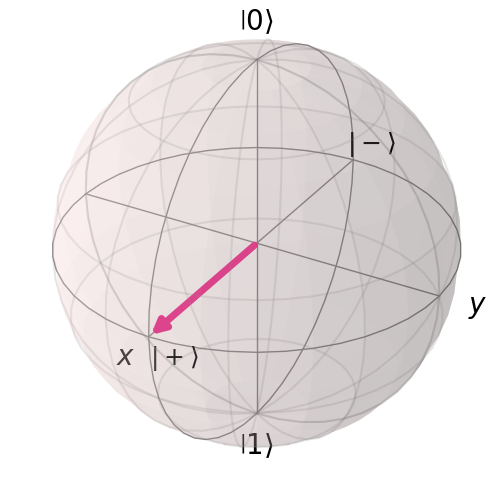
\includegraphics[width=\textwidth]{img/Bloch/bloch_state_+.png}
        \caption{Figura 13: Estado $|+\rangle$ en la esfera de Bloch. Obtenida de [Qiskit]}
    \end{minipage}
    \hfill
    \begin{minipage}{0.3\textwidth}
        \centering
        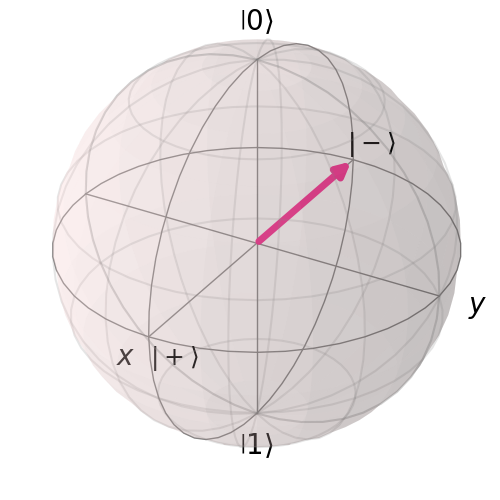
\includegraphics[width=\textwidth]{img/Bloch/bloch_state_-.png}
        \caption{Figura 14: Estado $|-\rangle$ en la esfera de Bloch. Obtenida de [Qiskit]}
    \end{minipage}
    \begin{minipage}{0.1\textwidth}
        \hfill
    \end{minipage}

    \vspace{5mm}

    Esto lo vimos en (\ref{eq: estados_eje_x_y}) cuando definimos los estados \( \ket{+} \) y \( \ket{-} \), y ahora hemos demostrado de donde salen. Estas son las puertas cuánticas de 1 qubit que principalmente vamos a usar, de manera que si aparece alguna otra puerta simple de 1 qubit la definiremos más adelante conforme nos vayan saliendo. Con esto damos por terminada esta sección y damos paso a la siguiente, en la que discutiremos qué sucede cuando tenemos más de 1 qubit\ldots



    






    \newpage
    \thispagestyle{empty}
    \mbox{}

    \section{Múltiples Qubits}\label{sec: multiples_qubits}

    \vspace{5mm}

    En esta sección, vamos a ver que se siguen las mismas reglas cuando tenemos más de un qubit que a la hora de tener solo uno, como vimos en la sección pasada (\ref{sec: el_qubit}). En este caso ya no estamos hablando de un qubit y por lo tanto, no nos encontramos en un espacio de Hilbert de dos dimensiones, sino que vamos a lograr generalizar las expresiones vistas en la sección anterior (\ref{sec: el_qubit}) para \( N \) qubits, llegando a las mismas expresiones que vimos en el espacio de Hilbert (\ref{sec: el_espacio_de_Hilbert}), y en este caso al tratarse de \( N \) qubits, tendríamos un espacio de Hilbert de \( 2^{N} \) dimensiones.


    \vspace{5mm}

    Para una mejor explicación, vamos a comenzar por un espacio de Hilbert de cuatro dimensiones, es decir, un sistema cuántico de dos qubits. Los estados de este sistema se pueden representar como

    \begin{equation*}
        \ket{0 0} = \ket{0} \otimes \ket{0} = \ket{0} \ket{0}
    \end{equation*}

    \vspace{2.5mm}

    Entonces, el resto de estados los podemos conseguir de la misma manera que sumamos números binarios, obteniendo que la base \( Z \) está formada por los siguientes estados

    \begin{equation*}
        Z = \{ \ket{0 0}, \ket{0 1}, \ket{1 0}, \ket{1 1} \}
    \end{equation*}

    \vspace{2.5mm}

    De manera que el estado de un qubit de carácter genérico es una superposición de estados en el eje \( Z \)

    \begin{equation}
        \ket{\psi} = c_{0} \ket{0 0} + c_{1} \ket{0 1} + c_{2} \ket{1 0} + c_{3} \ket{1 1}
        \label{eq: superposicion_qubit_2_estados}
    \end{equation}

    \vspace{2.5mm}

    Y las probabilidades de obtener los distintos estados \( \{ \ket{0 0}, \ket{0 1}, \ket{1 0}, \ket{1 1} \} \) al medir sobre el eje \( Z \) son \( | c_{0} |^{2} \), \( | c_{1} |^{2} \), \( | c_{2} |^{2} \) y \( | c_{3} |^{2} \), respectivamente. Hasta aquí no hay nada nuevo, pero ¿Qué sucede cuando queremos dar el paso a \( N \) qubits? Para esto necesitamos pasar los distintos estados de la base \( Z \) de binario a decimal. Suponiendo que los estados del eje \( Z \) se encuentran en la base binaria

    \begin{equation*}
        \ket{b_{N - 1} \ \cdots \ b_{2} \ b_{1} \ b_{0}}, \qquad \forall \ b_{n} \in \{0, 1\}
    \end{equation*}

    \vspace{2.5mm}

    Podemos realizar la conversión a decimal como sigue
    
    \begin{equation}
        \ket{b_{N - 1} \ \cdots \ b_{2} \ b_{1} \ b_{0}} = \ket{ 2^{N - 1} b_{N - 1} + \cdots + 2^{2} b_{2} + 2^{1} b_{1} + 2^{0} b_{0} }
        \label{eq: conversion_qubits_binario_decimal}
    \end{equation}

    \vspace{2.5mm}

    Y esta notación nos permite desarrollar el estado en superposición de un qubit \( \ket{\psi} \) que vimos en (\ref{eq: superposicion_qubit_2_estados}) cuando teníamos dos qubits, pero ahora teniendo \( N \) qubits

    \begin{equation}
        \ket{\psi} = \sum_{j = 0}^{N - 1} c_{j} \ket{j} = c_{0} \ket{0} + c_{1} \ket{1} + c_{2} \ket{2} + \cdots + c_{N - 1} \ket{N - 1}, \qquad j \in \mathbb{N} 
        \label{eq: estado_qubit_dimension_N}
    \end{equation}

    \vspace{2.5mm}

    Esta expresión nos resulta muy familiar, y es que ya la definimos anteriormente en (\ref{eq: combinacion_lineal_Hilbert}) cuando tratábamos los espacios de Hilbert (\ref{sec: el_espacio_de_Hilbert}), por lo que todo encaja muy bien y nos indica que vamos por buen camino. 

    \vspace{5mm}

    A continuación vamos a ver como es la representacón matricial de estos estados, y esto se hace con el denominado \textit{producto de Kronecker}, el cual no vamos a definirlo formalmente, sino que vamos a ver directamente como funciona, por ejemplo, para el estado \( \ket{0 0} \) en un sistema de dos qubits:

    \begin{equation*}
        \ket{0 0} = \ket{0} \ket{0} = \ket{0} \otimes \ket{0} = \begin{pmatrix}
            1 \\
            0
        \end{pmatrix} \otimes \begin{pmatrix}
            1 \\
            0
        \end{pmatrix} = \begin{pmatrix}
            1 \begin{pmatrix} 1 \\ 0 \end{pmatrix} \\
            0 \begin{pmatrix} 1 \\ 0 \end{pmatrix}
        \end{pmatrix} = \begin{pmatrix}
            1 \\
            0 \\
            0 \\
            0
        \end{pmatrix}
    \end{equation*}

    \vspace{2.5mm}

    Si esto lo aplicamos para el resto de estados que definen el eje \( Z \) en un sistema cuántico de dos qubits, obtenemos que

    \begin{equation}
        \ket{0 0} = \begin{pmatrix}
            1 \\
            0 \\
            0 \\
            0 
        \end{pmatrix}, \quad \ket{0 1} = \begin{pmatrix}
            0 \\
            1 \\
            0 \\
            0 
        \end{pmatrix}, \quad \ket{1 0} = \begin{pmatrix}
            0 \\
            0 \\
            1 \\
            0 
        \end{pmatrix}, \quad \ket{1 1} = \begin{pmatrix}
            0 \\
            0 \\
            0 \\
            1 
        \end{pmatrix}
        \label{eq: estados_matricial_2_qubits}
    \end{equation}

    \vspace{2.5mm}

    De manera que podemos expresar el estado de un sistema cuántico de dos qubits mediante un vector columna como vimos en (\ref{eq: vector_sistema_un_qubit}), ampliando la expresión para dos qubits y aplicando lo que acabamos de ver

    \begin{equation}
        \ket{\psi} = c_{0} \ket{0 0} + c_{1} \ket{0 1} + c_{2} \ket{1 0} + c_{3} \ket{1 1} = \begin{pmatrix}
            c_{0} \\
            c_{1} \\
            c_{2} \\
            c_{3}
        \end{pmatrix}
        \label{eq: estado_qubit_dimension_2_matriz}
    \end{equation}

    \vspace{2.5mm}

    Entonces, podemos representar la expresión (\ref{eq: estado_qubit_dimension_N}) como un vector columna de dimension \( N \), siendo \( N \) el número de qubits de nuestro sistema cuántico:

    \begin{equation}
        \ket{\psi} = \sum_{j = 0}^{N - 1} c_{j} \ket{j} = c_{0} \ket{0} + c_{1} \ket{1} + c_{2} \ket{2} + \cdots + c_{N - 1} \ket{N - 1} = \begin{pmatrix}
            c_{0} \\
            c_{1} \\
            c_{2} \\
            \vdots \\
            c_{N - 1}
        \end{pmatrix}
        \label{eq: estados_qubit_dimension_N_matriz}
    \end{equation}

    \vspace{2.5mm}

    Toda esta notación funciona exactamente igual para los bra, como por ejemplo \( \bra{0 0} \):

    \begin{equation*}
        \bra{0 0} = \bra{0} \otimes \bra{0} = \begin{pmatrix}
            1 & 0
        \end{pmatrix} \otimes \begin{pmatrix}
            1 & 0
        \end{pmatrix} = \begin{pmatrix}
            1 \begin{pmatrix} 1 & 0 \end{pmatrix} & 0 \begin{pmatrix} 1 & 0 \end{pmatrix}
        \end{pmatrix} = \begin{pmatrix}
            1 & 0 & 0 & 0
        \end{pmatrix}
    \end{equation*}

    \vspace{2.5mm}

    Entonces, de la misma manera que acabamos de ver en (\ref{eq: estados_qubit_dimension_N_matriz}) un ket generalizado para \( N \) qubits, ahora tenemos un bra generalizado para \( N \) qubits:

    \begin{equation}
        \bra{\psi} = \sum_{j = 0}^{N - 1} c_{j}^{*} \bra{j} = c_{0}^{*} \bra{0} + c_{1}^{*} \bra{1} + c_{2}^{*} \bra{2} + \cdots + c_{N - 1}^{*} \bra{N - 1} = \begin{pmatrix}
            c_{0}^{*} & c_{1}^{*} & c_{2}^{*} & \cdots & c_{N - 1}^{*}
        \end{pmatrix}
        \label{eq: bra_qubit_dimension_N_matriz}
    \end{equation}

    \vspace{10mm}

    


    \subsection{Puertas Cuánticas de Múltiples Qubits}

    \vspace{5mm}

    De la misma manera que vimos en las puertas cuánticas de un único qubit, las puertas cuánticas aplicadas a más de un qubit siguen siendo transformaciones del estado del qubit \( \ket{\psi} \) en otro \( \ket{\psi'} \), solo que ahora al tener más de una unidad de información cuántica no son rotaciones en la esfera de Bloch, y esto es porque no se pueda representar algo que esté más allá de las tres dimensiones, como vimos anteriormente en los estados de \( Z \) que eran vectores columna de cuatro elementos.

    \vspace{5mm}

    Vamos a comenzar creando algunas puertas de dos qubits. Aunque esto suene tedioso, es algo bastante sencillo si tenemos en cuenta lo que hemos visto anteriormente para puertas de un qubit en (\ref{subsection: puertas_cuanticas_de_1_qubit}), con la idea de que podemos aplicar cualquiera de estas transformaciones a los distintos qubits de \( \ket{\psi} \). Tomemos como ejemplo la puerta de Hadamard \textit{H} y la \textit{NOT} para un qubit, podemos aplicarlas a los distintos qubits de \( \ket{\psi} \), los cuales vamos a suponer que se encuentran en \( \ket{0 0} \)

    \begin{equation*}
        (H \otimes X) \ket{\psi} = (H \otimes X) \ket{0 0} = (H \otimes X) \ket{0} \otimes \ket{0} = H \ket{0} \otimes X \ket{0} = \ket{+} \otimes \ket{1} = \frac{1}{\sqrt{2}} \left( \ket{0} + \ket{1} \right) \otimes \ket{1} =
    \end{equation*}
    \begin{equation*}
        = \frac{1}{\sqrt{2}} \left( \ket{0} \otimes \ket{1} + \ket{1} \otimes \ket{1} \right) = \frac{1}{\sqrt{2}} \left( \ket{0 1} + \ket{1 1} \right)
    \end{equation*}

    \vspace{2.5mm}

    Y de esta manera podemos ver perfectamente que se ha aplicado una puerta \textit{H} al qubit en la izquierda y una puerta \textit{X} al qubit de la derecha. Este resultado también lo podemos obtener matricialmente ya que \( \otimes \) es el producto de Kronecker. Vamos a definir primero la matriz que representa esta puerta cuántica

    \begin{equation*}
        H \otimes X = \frac{1}{\sqrt{2}} \begin{pmatrix}
            1 & 1 \\
            1 & -1 
        \end{pmatrix} \otimes \begin{pmatrix}
            0 & 1 \\
            1 & 0 
        \end{pmatrix} = \frac{1}{\sqrt{2}} \begin{pmatrix}
            1 \begin{pmatrix} 0 & 1 \\ 1 & 0 \end{pmatrix} & 1 \begin{pmatrix} 0 & 1 \\ 1 & 0 \end{pmatrix} \\  
            1 \begin{pmatrix} 0 & 1 \\ 1 & 0 \end{pmatrix} & -1 \begin{pmatrix} 0 & 1 \\ 1 & 0 \end{pmatrix}
        \end{pmatrix} = \frac{1}{\sqrt{2}} \begin{pmatrix}
            0 & 1 & 0 & 1 \\
            1 & 0 & 1 & 0 \\
            0 & 1 & 0 & -1 \\
            1 & 0 & -1 & 0
        \end{pmatrix}
    \end{equation*}

    \vspace{2.5mm}

    Vemos que esta matriz es unitaria, por lo que se verifica que es una puerta cuántica perfectamente válida. Entonces, si multiplicamos esta matriz por el estado \( \ket{0 0} \) de \( \ket{\psi} \) obtenemos, como debería de ser, el mismo resultado

    \begin{equation*}
        \left( H \otimes X \right) \ket{0 0} =  \frac{1}{\sqrt{2}} \begin{pmatrix}
            0 & 1 & 0 & 1 \\
            1 & 0 & 1 & 0 \\
            0 & 1 & 0 & -1 \\
            1 & 0 & -1 & 0
        \end{pmatrix} \begin{pmatrix}
            1 \\
            0 \\
            0 \\
            0
        \end{pmatrix} = \frac{1}{\sqrt{2}} \begin{pmatrix}
            0 \\ 
            1 \\
            0 \\
            1
        \end{pmatrix} = \frac{1}{\sqrt{2}} \left( \ket{0 1} + \ket{1 1} \right)
    \end{equation*}

    \vspace{2.5mm}

    Y así podemos crear nuestras propias puertas cuánticas a nuestro gusto, según nuestras propias necesidades, asegurándonos siempre que sean puertas válidas. Volveremos a este ejemplo más adelante, ya que como veremos, aplicar puertas cuánticas simples de un qubit a un estado con múltiples qubits no puede crear el famoso entrelazamiento cuántico, el cual explicaremos detenidamente en (\ref{sec: entrelazamiento_cuantico}). Sin embargo, podemos tener puertas cuánticas que cambien directamente el estado de dos qubits al mismo tiempo, al contrario de las puertas que hemos visto hasta ahora, y estas son de vital importancia ya que sí permiten crear entrelazamiento. 

    \vspace{10mm}





    \newpage
    \thispagestyle{empty}
    \mbox{}

    \section{Errores Cuánticos}
    \subsection{Decoherencia}
    \subsection{Shor Code}





    \newpage
    \thispagestyle{empty}
    \mbox{}

    \section{Entrelazamiento Cuántico}\label{sec: entrelazamiento_cuantico}
    \subsection{Estados de Bell}
    \subsection{Codificación Superdensa}
    \subsection{Teleportación Cuántica}





    \newpage
    \thispagestyle{empty}
    \mbox{}

    \section{Algoritmos Cuánticos}\label{sec: algoritmos_cuanticos}
    \subsection{Oracles Cuánticos}
    \subsection{Algoritmo de Grover}
    \subsection{Algoritmo de Shor}





    \newpage
    \thispagestyle{empty}
    \mbox{}

    \section{Estado del Arte}

    \vspace{5mm}

    La empresa líder en computación cuántica es, hasta la fecha y sin duda alguna, IBM, la cual ofrece a nuestra disposición distintas páginas web en las que podemos ejecutar circuitos cuánticos y ver su comportamiento de la manera más real posible. El desarrollo del circuito se hace a través de \textit{Python} mediante su librería destinada a la computación cuántica \textit{Qiskit}, y una vez lo hemos completado, tenemos distintas opciones de configuración para la ejecución del circuito.

    \vspace{5mm}

    Por otra parte, si la programación en \textit{Python} no es nuestro punto fuerte, tenemos a nuestra disposición la interfaz gráfica para el desarrollo de circuitos cuánticos de IBM, Quantum Composer. Con esta herramiento web podemos crear circuitos cuánticos con el sistema \textit{drag and drop} sobre puertas cuánticas o qubits, de manera que se genera el correspondiente código equivalente al circuito cuántico creado y se ejecuta en un emulador o sistema cuántico, además de que podemos visualizar el estado y la fase correspondiente en la \textit{esfera de Bloch}, y un histograma con las probabilidades de los estados a los que puede colapsar el circuito.
    
    \vspace{5mm}

    De la misma manera que IBM, Amazon ha desarrollado su propia plataforma para la ejecución de circuitos cuánticos, la cual está basada nuevamente en \textit{Python}, con la diferencia de que usamos la librería relacionada con su propio producto, \textit{Braket}. Este producto incluye ciertas ventajas sobre el producto de IBM, como que permite la combinación de computación cuántica y clásica, aunque como vimos anteriormente, todo circuito clásico se puede expresar como un circuito cuántico. Tambień podemos encontrar productos de otras empresas para la simulación y ejecución de circuitos cuánticos, como Google o Azure, pero no dejan de ser, junto con el producto de Amazon, competidores de la solución presentada por IBM, la cual fue la primera en salir públicamente al mercado con su plataforma IBM Quantum Experience, lanzada en \textit{2016}.

    \vspace{5mm}

    No obstante, la computación cuántica tiene muchos problemas, relacionados precisamente con la naturaleza de las partículas subatómicas, las cuales son muy sensibles al ruido causado por el exterior, lo que hace que se produzcan muchos fallos en los circuitos y que, por lo tanto, los computadores cuánticos actuales no sean tolerantes a fallos (\textit{fault-tolerant}), de manera que los errores se acumulan muy rápidamente y sin la capacidad de ser revertidos con la tecnología cuántica hasta el momento. Sin embargo, Microsoft ha hecho un hallazgo que puede convertirse en la revolución del siglo, mucho más allá que el desarrollo de la inteligencia artificial en estos últimos años.

    \vspace{5mm}

    Microsoft ha anunciado el lanzamiento de \textit{Majorana 1}, la primera unidad de procesamiento cuántico (QPU) con qubits topológicos, qubits que almacenan informacion cuántica de manera más estable y robusta, de manera que es mucho menos susceptible a errores cuánticos, que es uno de los principales problemas de este campo de la física y la tecnología, siendo una de las principales motivaciones para Microsoft construir el primer ordenador cuántico con tolerancia a fallos en los próximos años.

    \vspace{5mm}

    La clave de este gran avance ha sido el desarrollo de materiales topoconductores, los cuales permiten la superconductividad topológica, un estado de la materia que hasta este descubrimiento solo existía en la teoría. Este tipo de materiales se crean con arseniuro de indio y aluminio, de manera que cuando se enfrían prácticamente al cero aboluto y se sintonizan con campos magnéticos, se forman nanocables superconductores topológicos con modos cero de Majorana (MZM) en sus extremos, de manera que aumentan la estabilidad y se reducen los errores en comparación con los qubits tradicionales.
    \vspace{5mm}

    Así es como se ha desarrollado el primer qubit topológico del mundo, y se plantea tener un chip cuántico con más de un millón de qubits y tolerante a fallos en unos años, y no en unas décadas como se planteaba anteriormente, dando un gran paso en la computación cuántica práctica y probablemente uno de los mayores hitos de este campo.





    % Pagina en blanco
    \newpage
    \thispagestyle{empty}
    \mbox{}
    \newpage

    \section{Bibliografía}

        \vspace{5mm}

        TFG Silvia Rodriguez\par
        \url{https://matematicas.uam.es/~fernando.chamizo/supervision/TFG/past/memoirs/TFG_silvia_rodriguez.pdf}
        \vspace{2mm}

        Investigacion Computacion Cuantica --> Seguridad informatica, redes informaticas, IA, etc.\par
        \url{https://rua.ua.es/dspace/bitstream/10045/124691/1/Estudio_de_la_computacion_cuantica_en_los_diferent_Claramunt_Carriles_Sergio.pdf}
        \vspace{2mm}

        Universidad de Murcia --> Schrodinguer, Hamiltoniano, Oscilador armonico, Atomo de Hidrogeno\par
        \url{https://webs.um.es/gustavo.garrigos/tfg/MarinMunoz_Diego_TFG_julio2021.pdf}
        \vspace{2mm}

        TFG Pablo --> Algoritmo de Grover y otros algoritmos\par
        \url{https://rodin.uca.es/bitstream/handle/10498/27218/tfg_pablo.pdf}
        \vspace{2mm}

        TFM --> Schrodinguer e interpretacion probabilistica de la funcion de onda\par
        \url{https://repositorioinstitucional.buap.mx/server/api/core/bitstreams/fb9bfe95-7945-404d-a3c5-00ba77b8ad71/content}
        \vspace{2mm}

        Universidad Autonoma de Madrid --> Interpretacion probabilistica de la funcion de onda e introduccion al atomo de hidrogeno\par
        \url{https://matematicas.uam.es/~fernando.chamizo/supervision/TFG/past/memoirs/TFG_luis_sanchez.pdf}
        \vspace{2mm}

        TFG --> Espacios de Hilbert y su relacion con la mecanica cuantica\par
        \url{https://idus.us.es/server/api/core/bitstreams/4c49766a-cdfc-4d72-9acf-f62761db63fb/content}
        \vspace{2mm}

        Claudia Mielgo --> El sistema cuantico es un espacio de Hilbert, y funciones de onda\par
        \url{https://matematicas.uam.es/~fernando.chamizo/supervision/TFG/past/memoirs/TFG_claudia_mielgo.pdf}
        \vspace{2mm}

        Algebra Lineal --> Algebra lineal, espacios de Hilbert y criptografia cuantica\par
        \url{https://repositorio.ual.es/bitstream/handle/10835/9810/VILLASANA%20ALCARAZ%2C%20MARIA%20DEL%20MAR.pdf}
        \vspace{2mm}

        Roberto Gonzalez --> Sistema Bineario e introduccion a los qubits\par
        \url{https://oa.upm.es/69234/1/TFG_ROBERTO_GONZALEZ_RIVAS.pdf}
        \vspace{2mm}

        Por que un ordenador cuantico?\par
        \url{https://zaguan.unizar.es/record/76803/files/TAZ-TFG-2018-3072.pdf}
        \vspace{2mm}

        Radiacion del cuerpo negro\par
        \url{https://www.fisicacuantica.es/la-radiacion-del-cuerpo-negro/}
        \vspace{2mm}

        \url{https://weblab.deusto.es/olarex/cd/kaernten/BBR_ES_new_27.09.2013/distribucin_de_la_energa.html}
        \vspace{2mm}

        \url{https://www.quimicafisica.com/teoria-cuantica/la-radiacion-del-cuerpo-negro.html}
        \vspace{2mm}

        Efecto Fotoeléctrico\par
        \url{https://es.khanacademy.org/science/ap-chemistry/electronic-structure-of-atoms-ap/bohr-model-hydrogen-ap/a/photoelectric-effect}
        \vspace{2mm}

        \url{https://www.quimicafisica.com/teoria-cuantica/el-efecto-fotoelectrico.html}
        \vspace{2mm}

        Experimento de la Doble Rendija\par
        \url{https://www.fisicalab.com/apartado/cantidad-movimiento#google_vignette}
        \vspace{2mm}

        \url{https://www.dciencia.es/fisica-cuantica-el-experimento-de-la-doble-rendija/}
        \vspace{2mm}

        \url{https://mecanicosvalencia.es/max-born-mecanica-cuantica/}
        \vspace{2mm}

        Espacios de Hilbert. El concepto de espacio de Hilbert es una generalización del concepto de espacio euclídeo.\par
        \url{https://uvadoc.uva.es/bitstream/handle/10324/57982/TFG-G5986.pdf?sequence=1}
        \vspace{2mm}

        \url{https://ecfm.usac.edu.gt/sites/default/files/2021-06/Joel%20Armando%20Ju%C3%A1rez.pdf}
        \vspace{2mm}

        \url{https://repositorio.ual.es/bitstream/handle/10835/9810/VILLASANA%20ALCARAZ%2C%20MARIA%20DEL%20MAR.pdf}
        \vspace{2mm}

        Videos espacios de Hilbert\par
        \url{https://www.youtube.com/watch?v=ZfZ39YpHZE0}
        \vspace{2mm}

        \url{https://www.youtube.com/watch?v=sZ5lwXuD5mA&t=1057s}
        \vspace{2mm}

        \url{https://campusvirtual.ull.es/ocw/file.php/26/tema1/1-ehilbert.pdf}
        \vspace{2mm}

        Majorana\par
        \url{https://news.microsoft.com/source/latam/noticias-de-microsoft/microsoft-presenta-majorana-1-el-primer-procesador-cuantico-del-mundo-impulsado-por-qubits-topologicos/}
        \vspace{2mm}

        Postulados\par
        \url{https://uvadoc.uva.es/bitstream/handle/10324/70993/TFG-G6793.pdf}
        \vspace{2mm}

        \url{https://idus.us.es/server/api/core/bitstreams/e6e34b3a-fc74-4043-98ae-8244902b96e4/content}
        \vspace{2mm}

        Espacio L2 \\
        \url{https://uvadoc.uva.es/bitstream/handle/10324/44929/TFG-G4732.pdf}

    
\end{document}